\PassOptionsToPackage{unicode=true}{hyperref} % options for packages loaded elsewhere
\PassOptionsToPackage{hyphens}{url}
%
\documentclass[10pt,xcolor=table,color={dvipsnames,usenames},ignorenonframetext,usepdftitle=false,french]{beamer}
\setbeamertemplate{caption}[numbered]
\setbeamertemplate{caption label separator}{: }
\setbeamercolor{caption name}{fg=normal text.fg}
\beamertemplatenavigationsymbolsempty
\usepackage{caption}
\captionsetup{skip=0pt,belowskip=0pt}
%\setlength\abovecaptionskip{-15pt}
\usepackage{lmodern}
\usepackage{amssymb,amsmath,mathtools,multirow}
\usepackage{float,hhline}
\usepackage{tikz}
\usepackage{mathtools}
\usepackage{ifxetex,ifluatex}
\usepackage{fixltx2e} % provides \textsubscript
\ifnum 0\ifxetex 1\fi\ifluatex 1\fi=0 % if pdftex
  \usepackage[T1]{fontenc}
  \usepackage[utf8]{inputenc}
  \usepackage{textcomp} % provides euro and other symbols
\else % if luatex or xelatex
  \usepackage{unicode-math}
  \defaultfontfeatures{Ligatures=TeX,Scale=MatchLowercase}
\fi
\usetheme[coding=utf8,language=french,
,titlepagelogo=img/logobeamer.png
]{TorinoTh}
% use upquote if available, for straight quotes in verbatim environments
\IfFileExists{upquote.sty}{\usepackage{upquote}}{}
% use microtype if available
\IfFileExists{microtype.sty}{%
\usepackage[]{microtype}
\UseMicrotypeSet[protrusion]{basicmath} % disable protrusion for tt fonts
}{}
\IfFileExists{parskip.sty}{%
\usepackage{parskip}
}{% else
\setlength{\parindent}{0pt}
\setlength{\parskip}{6pt plus 2pt minus 1pt}
}
\usepackage{hyperref}
\hypersetup{
            pdfauthor={Alain Quartier-la-Tente},
            pdfborder={0 0 0},
            breaklinks=true}
\urlstyle{same}  % don't use monospace font for urls
\newif\ifbibliography
\newlength{\cslhangindent}
\setlength{\cslhangindent}{1.5em}
\newlength{\csllabelwidth}
\setlength{\csllabelwidth}{3em}
\newenvironment{CSLReferences}[2] % #1 hanging-ident, #2 entry spacing
 {% don't indent paragraphs
  \setlength{\parindent}{0pt}
  % turn on hanging indent if param 1 is 1
  \ifodd #1 \everypar{\setlength{\hangindent}{\cslhangindent}}\ignorespaces\fi
  % set entry spacing
  \ifnum #2 > 0
  \setlength{\parskip}{#2\baselineskip}
  \fi
 }%
 {}
\usepackage{color}
\usepackage{fancyvrb}
\newcommand{\VerbBar}{|}
\newcommand{\VERB}{\Verb[commandchars=\\\{\}]}
\DefineVerbatimEnvironment{Highlighting}{Verbatim}{commandchars=\\\{\}}
% Add ',fontsize=\small' for more characters per line
\usepackage{framed}
\definecolor{shadecolor}{RGB}{248,248,248}
\newenvironment{Shaded}{\begin{snugshade}}{\end{snugshade}}
\newcommand{\AlertTok}[1]{\textcolor[rgb]{0.94,0.16,0.16}{#1}}
\newcommand{\AnnotationTok}[1]{\textcolor[rgb]{0.56,0.35,0.01}{\textbf{\textit{#1}}}}
\newcommand{\AttributeTok}[1]{\textcolor[rgb]{0.13,0.29,0.53}{#1}}
\newcommand{\BaseNTok}[1]{\textcolor[rgb]{0.00,0.00,0.81}{#1}}
\newcommand{\BuiltInTok}[1]{#1}
\newcommand{\CharTok}[1]{\textcolor[rgb]{0.31,0.60,0.02}{#1}}
\newcommand{\CommentTok}[1]{\textcolor[rgb]{0.56,0.35,0.01}{\textit{#1}}}
\newcommand{\CommentVarTok}[1]{\textcolor[rgb]{0.56,0.35,0.01}{\textbf{\textit{#1}}}}
\newcommand{\ConstantTok}[1]{\textcolor[rgb]{0.56,0.35,0.01}{#1}}
\newcommand{\ControlFlowTok}[1]{\textcolor[rgb]{0.13,0.29,0.53}{\textbf{#1}}}
\newcommand{\DataTypeTok}[1]{\textcolor[rgb]{0.13,0.29,0.53}{#1}}
\newcommand{\DecValTok}[1]{\textcolor[rgb]{0.00,0.00,0.81}{#1}}
\newcommand{\DocumentationTok}[1]{\textcolor[rgb]{0.56,0.35,0.01}{\textbf{\textit{#1}}}}
\newcommand{\ErrorTok}[1]{\textcolor[rgb]{0.64,0.00,0.00}{\textbf{#1}}}
\newcommand{\ExtensionTok}[1]{#1}
\newcommand{\FloatTok}[1]{\textcolor[rgb]{0.00,0.00,0.81}{#1}}
\newcommand{\FunctionTok}[1]{\textcolor[rgb]{0.13,0.29,0.53}{\textbf{#1}}}
\newcommand{\ImportTok}[1]{#1}
\newcommand{\InformationTok}[1]{\textcolor[rgb]{0.56,0.35,0.01}{\textbf{\textit{#1}}}}
\newcommand{\KeywordTok}[1]{\textcolor[rgb]{0.13,0.29,0.53}{\textbf{#1}}}
\newcommand{\NormalTok}[1]{#1}
\newcommand{\OperatorTok}[1]{\textcolor[rgb]{0.81,0.36,0.00}{\textbf{#1}}}
\newcommand{\OtherTok}[1]{\textcolor[rgb]{0.56,0.35,0.01}{#1}}
\newcommand{\PreprocessorTok}[1]{\textcolor[rgb]{0.56,0.35,0.01}{\textit{#1}}}
\newcommand{\RegionMarkerTok}[1]{#1}
\newcommand{\SpecialCharTok}[1]{\textcolor[rgb]{0.81,0.36,0.00}{\textbf{#1}}}
\newcommand{\SpecialStringTok}[1]{\textcolor[rgb]{0.31,0.60,0.02}{#1}}
\newcommand{\StringTok}[1]{\textcolor[rgb]{0.31,0.60,0.02}{#1}}
\newcommand{\VariableTok}[1]{\textcolor[rgb]{0.00,0.00,0.00}{#1}}
\newcommand{\VerbatimStringTok}[1]{\textcolor[rgb]{0.31,0.60,0.02}{#1}}
\newcommand{\WarningTok}[1]{\textcolor[rgb]{0.56,0.35,0.01}{\textbf{\textit{#1}}}}
% Prevent slide breaks in the middle of a paragraph:
\widowpenalties 1 10000
\raggedbottom
\AtBeginPart{
  \let\insertpartnumber\relax
  \let\partname\relax
  \frame{\partpage}
}
\AtBeginSection{
  \ifbibliography
  \else
    \begin{frame}{Sommaire}
    \tableofcontents[currentsection, hideothersubsections]
    \end{frame}
  \fi
}
\setlength{\emergencystretch}{3em}  % prevent overfull lines
\providecommand{\tightlist}{%
  %\setlength{\itemsep}{0pt}
  \setlength{\parskip}{0pt}
  }
\setcounter{secnumdepth}{0}

% set default figure placement to htbp
\makeatletter
\def\fps@figure{htbp}
\makeatother

\usepackage{dsfont}
\usepackage{stmaryrd}
\usepackage[normalem]{ulem}
\usepackage{fontawesome5}
\usepackage{tikz,pgfplots}
\pgfplotsset{compat=1.17}
\pgfplotsset{samples=100}
\usepackage{animate}
 \usepackage{booktabs}

\usepackage{colortbl}

\DeclareMathOperator{\Cov}{Cov}
\newcommand{\cov}[2]{\Cov\left( #1\,,\,#2 \right)}

\DeclareMathOperator{\e}{e}
\renewcommand{\P}{\mathds{P}} %Apparement \P existe déjà ?
\newcommand\N{\mathds{N}}
\newcommand\R{\mathds{R}}


\newcommand\1{\mathds{1}}
\newcommand{\E}[2][]{{\mathds{E}}_{#1}
  \def\temp{#2}\ifx\temp\empty
  \else
    \left[#2\right]
  \fi
}
\newcommand{\V}[2][]{{\mathds{V}}_{#1}
  \def\temp{#2}\ifx\temp\empty
  \else
    \left[#2\right]
  \fi
}
\newcommand\ud{\,\mathrm{d}}


% blocks
\usepackage{environ}
\usepackage[tikz]{bclogo}

\tikzstyle{titlestyle} =[draw=black!80,fill=black!20, text=black,
 right=10pt, rounded corners]
\mdfdefinestyle{symmaryboxstyle}{
	linecolor=black!80, backgroundcolor = black!5,
	skipabove=\baselineskip, innertopmargin=\baselineskip,
	innerbottommargin=\baselineskip,
	userdefinedwidth=\textwidth,
	middlelinewidth=1.2pt, roundcorner=5pt,
	skipabove={\dimexpr0.5\baselineskip+\topskip\relax},
	frametitleaboveskip=\dimexpr-\ht\strutbox\relax,
	innerlinewidth=0pt,
}
\NewEnviron{summary}{%
\begin{mdframed}[style=symmaryboxstyle]
\vspace{-0.5em}
\BODY
\end{mdframed}
}
\makeatletter
% Open `\noalign` and check for overlay specification:
\def\rowcolor{\noalign{\ifnum0=`}\fi\bmr@rowcolor}
\newcommand<>{\bmr@rowcolor}{%
    \alt#1%
        {\global\let\CT@do@color\CT@@do@color\@ifnextchar[\CT@rowa\CT@rowb}% Rest of original `\rowcolor`
        {\ifnum0=`{\fi}\@gooble@rowcolor}% End `\noalign` and gobble all arguments of `\rowcolor`.
}
% Gobble all normal arguments of `\rowcolor`:
\newcommand{\@gooble@rowcolor}[2][]{\@gooble@rowcolor@}
\newcommand{\@gooble@rowcolor@}[1][]{\@gooble@rowcolor@@}
\newcommand{\@gooble@rowcolor@@}[1][]{\ignorespaces}

\newcommand{\rowc}[1]{\only<#1>{\\\rowcolor{processblue!40}}}
%\newcommand{\rowc}[1]{{\rowcolor<#1>{processblue!30}}
\newcommand{\cellc}[1]{\only<#1>{\cellcolor{processblue!40}}}
\newcommand{\supsp}[1]{\visible<#1>{\\}}

\title{Estimation en temps réel de la tendance-cycle :\\
Apport de l'utilisation des filtres asymétriques dans la détection des
points de retournement}
\ateneo{CSI}
\author{Alain Quartier-la-Tente}
\date{}


\setrellabel{}

\setcandidatelabel{}

\rel{}
\division{}

\departement{08 novembre 2023}
\makeatletter
\let\@@magyar@captionfix\relax
\makeatother


\begin{document}
\begin{frame}[plain,noframenumbering]
\titlepage
\end{frame}

\hypertarget{introduction}{%
\section{Introduction}\label{introduction}}

\begin{frame}{Présentation}
\protect\hypertarget{pruxe9sentation}{}
Travaille à l'Insee depuis 2015 : aux enquêtes de conjoncture
(2015-2017), en tant que méthodologue sur les CVS-CJO (2017-2019) puis
en tant que chargé d'études macroéconomiques (2021-)

Ensai (2012-2015) puis Ensae (2019-2021) et inscription en thèse à temps
partiel en 2021

\pause

Passionné de \faIcon{r-project}, développe et maintien plusieurs
packages autour de la désaisonnalisation
\end{frame}

\begin{frame}[fragile]{Travaux effectués}
\protect\hypertarget{travaux-effectuuxe9s}{}
Principalement autour de l'utilisation de moyennes mobiles asymétriques
pour l'estimation en temps réel de la tendance-cycle et la détection des
points de retounement.

\begin{itemize}
\item
  Un document de travail Insee en cours avec code ouvert et entièrement
  reproductible, pour l'instant disponible ici
  \url{https://aqlt.github.io/DT-est-tr-tc/}
\item
  Une soumission en cours au Journal of Official Statistics (JOS).
\item
  Un package \texttt{rjd3filters} pour créer et manipuler les moyennes
  mobiles
\item
  Divers présentations sur le contenu statistique et informatique.
\end{itemize}

\pause

NB : études rédigées seul
\end{frame}

\begin{frame}{La tendance-cycle (1)}
\protect\hypertarget{la-tendance-cycle-1}{}
\(X_t\) (ex : IPI France) se décompose en plusieurs composantes
inobservées : \[
X_t=\onslide<2->{\underbrace{TC_t}_{\text{tendance-cycle}}}
\onslide<3->{
+\underbrace{S_t}_{\text{saisonnalité}}
}
\onslide<4->{
+\underbrace{I_t}_{\text{irrégulier}}
}
\text{ (décomposition additive)}
\] \onslide<5>{tendance et cycle ici estimés \highlight{simultanément}}

\begin{tikzpicture}
\begin{axis}[enlarge x limits=false, ylabel={IPI France},ymin = 66,ymax=120, 
xtick={2010,2012,...,2020}, xticklabels={2010,2012,...,2020},width=\textwidth, height=0.7\textheight]
\only<1->{
\addplot[mark=none, black] coordinates {(2010,90.3) (2010.083,93.1) (2010.167,109.5) (2010.25,100.4) (2010.333,95.5) (2010.417,111.8) (2010.5,100.8) (2010.583,74.5) (2010.667,109) (2010.75,105) (2010.833,102.7) (2010.917,101.9) (2011,99) (2011.083,101.6) (2011.167,115.3) (2011.25,101.6) (2011.333,110.1) (2011.417,108.5) (2011.5,101) (2011.583,78.3) (2011.667,110) (2011.75,106.4) (2011.833,106.3) (2011.917,100.2) (2012,99.3) (2012.083,99.9) (2012.167,110.3) (2012.25,99.8) (2012.333,96.1) (2012.417,108.5) (2012.5,103.8) (2012.583,78.8) (2012.667,102.9) (2012.75,107.6) (2012.833,101.9) (2012.917,91.5) (2013,96.3) (2013.083,95.7) (2013.167,103.9) (2013.25,103.4) (2013.333,96.2) (2013.417,105.5) (2013.5,105.2) (2013.583,73.4) (2013.667,103.3) (2013.75,109.3) (2013.833,99) (2013.917,94.6) (2014,96.8) (2014.083,97.1) (2014.167,104.9) (2014.25,102.9) (2014.333,92.4) (2014.417,104.8) (2014.5,103.3) (2014.583,71.5) (2014.667,107.2) (2014.75,107.7) (2014.833,95.5) (2014.917,98.4) (2015,94.6) (2015.083,96.1) (2015.167,108.4) (2015.25,102.4) (2015.333,91) (2015.417,111.8) (2015.5,101.1) (2015.583,76.1) (2015.667,109.1) (2015.75,107.7) (2015.833,101.8) (2015.917,99.9) (2016,95.1) (2016.083,99.6) (2016.167,108.3) (2016.25,103.3) (2016.333,98.6) (2016.417,110.3) (2016.5,95.8) (2016.583,79.7) (2016.667,107.9) (2016.75,103.4) (2016.833,104.7) (2016.917,99.7) (2017,98.9) (2017.083,97.1) (2017.167,114.5) (2017.25,98) (2017.333,102.7) (2017.417,111.4) (2017.5,99.5) (2017.583,81.4) (2017.667,108.2) (2017.75,113.2) (2017.833,111) (2017.917,99.5) (2018,101.8) (2018.083,98.6) (2018.167,112.9) (2018.25,103) (2018.333,98.7) (2018.417,112.8) (2018.5,106.6) (2018.583,82.6) (2018.667,104.7) (2018.75,116) (2018.833,109.6) (2018.917,97.6) (2019,103.8) (2019.083,102) (2019.167,111.6) (2019.25,107.2) (2019.333,105.2) (2019.417,106) (2019.5,109.8) (2019.583,78.8) (2019.667,109) (2019.75,116.5) (2019.833,104) (2019.917,97.8) (2020,101) (2020.083,100.1) (2020.167,91.8) (2020.25,66.7) (2020.333,73.7) (2020.417,98.2) (2020.5,97.4) (2020.583,71.7) (2020.667,104.7) (2020.75,106.7) (2020.833,101.6) (2020.917,96.6)};}
\only<2->{
\addplot+[mark=none,blue] coordinates {(2010,96.6) (2010.083,97.1) (2010.167,97.9) (2010.25,98.9) (2010.333,99.7) (2010.417,100.2) (2010.5,100.3) (2010.583,100.4) (2010.667,100.5) (2010.75,101) (2010.833,101.9) (2010.917,102.8) (2011,103.4) (2011.083,103.7) (2011.167,103.5) (2011.25,102.8) (2011.333,102.1) (2011.417,101.5) (2011.5,101.2) (2011.583,101.4) (2011.667,101.7) (2011.75,102.1) (2011.833,102.4) (2011.917,102.4) (2012,102.1) (2012.083,101.6) (2012.167,101) (2012.25,100.6) (2012.333,100.4) (2012.417,100.4) (2012.5,100.4) (2012.583,100.2) (2012.667,99.6) (2012.75,99) (2012.833,98.4) (2012.917,98) (2013,98) (2013.083,98.3) (2013.167,98.8) (2013.25,99.2) (2013.333,99.4) (2013.417,99.4) (2013.5,99.2) (2013.583,98.9) (2013.667,98.6) (2013.75,98.4) (2013.833,98.4) (2013.917,98.5) (2014,98.7) (2014.083,98.9) (2014.167,98.8) (2014.25,98.7) (2014.333,98.5) (2014.417,98.3) (2014.5,98.2) (2014.583,98.1) (2014.667,98.2) (2014.75,98.2) (2014.833,98.3) (2014.917,98.5) (2015,98.7) (2015.083,99.1) (2015.167,99.4) (2015.25,99.8) (2015.333,100.3) (2015.417,100.7) (2015.5,101) (2015.583,101.3) (2015.667,101.3) (2015.75,101.2) (2015.833,101) (2015.917,100.7) (2016,100.6) (2016.083,100.6) (2016.167,100.7) (2016.25,100.8) (2016.333,100.8) (2016.417,100.8) (2016.5,100.6) (2016.583,100.4) (2016.667,100.3) (2016.75,100.5) (2016.833,100.9) (2016.917,101.5) (2017,102) (2017.083,102.3) (2017.167,102.4) (2017.25,102.3) (2017.333,102) (2017.417,101.9) (2017.5,102.3) (2017.583,102.9) (2017.667,103.7) (2017.75,104.4) (2017.833,104.7) (2017.917,104.6) (2018,104) (2018.083,103.4) (2018.167,103.1) (2018.25,103.1) (2018.333,103.3) (2018.417,103.6) (2018.5,103.9) (2018.583,104) (2018.667,104.2) (2018.75,104.4) (2018.833,104.7) (2018.917,105.1) (2019,105.5) (2019.083,105.8) (2019.167,105.9) (2019.25,105.7) (2019.333,105.4) (2019.417,105) (2019.5,104.6) (2019.583,104.2) (2019.667,103.7) (2019.75,103.4) (2019.833,103.2) (2019.917,103.1) (2020,103) (2020.083,103) (2020.167,103.2) (2020.25,103.6) (2020.333,104) (2020.417,104.4) (2020.5,104.5) (2020.583,104.4) (2020.667,103.9) (2020.75,103.3) (2020.833,102.8) (2020.917,102.5)};
}
\only<3->{
\addplot+[mark=none,green!60!black] coordinates {(2010,91) (2010.083,93.7) (2010.167,109.5) (2010.25,99.9) (2010.333,92.4) (2010.417,111.9) (2010.5,101.7) (2010.583,73.8) (2010.667,108.9) (2010.75,106) (2010.833,106.1) (2010.917,102.4) (2011,97.5) (2011.083,100.5) (2011.167,114.7) (2011.25,102.4) (2011.333,97) (2011.417,111.9) (2011.5,101.1) (2011.583,78.6) (2011.667,109.8) (2011.75,106.4) (2011.833,106.7) (2011.917,99.1) (2012,98.6) (2012.083,101.8) (2012.167,109.9) (2012.25,99.8) (2012.333,97.3) (2012.417,108.9) (2012.5,102.7) (2012.583,77.6) (2012.667,103.1) (2012.75,108.7) (2012.833,101.3) (2012.917,92.2) (2013,96.8) (2013.083,95.4) (2013.167,103.4) (2013.25,103.9) (2013.333,96.2) (2013.417,104.9) (2013.5,104.6) (2013.583,74.2) (2013.667,104) (2013.75,107.5) (2013.833,99.4) (2013.917,95.2) (2014,97.4) (2014.083,95.9) (2014.167,105.4) (2014.25,101.6) (2014.333,92.9) (2014.417,105.9) (2014.5,102.9) (2014.583,71.8) (2014.667,106.1) (2014.75,107.5) (2014.833,96.6) (2014.917,98.2) (2015,94.7) (2015.083,95.8) (2015.167,108.3) (2015.25,101.8) (2015.333,93.4) (2015.417,110.9) (2015.5,105.4) (2015.583,74.9) (2015.667,109.4) (2015.75,108.1) (2015.833,101.7) (2015.917,99.9) (2016,94.6) (2016.083,99.7) (2016.167,109.5) (2016.25,103) (2016.333,96.6) (2016.417,110.7) (2016.5,100.2) (2016.583,79.4) (2016.667,107.1) (2016.75,105.6) (2016.833,105.3) (2016.917,98) (2017,98.1) (2017.083,98.3) (2017.167,113.5) (2017.25,98.8) (2017.333,101.3) (2017.417,111.8) (2017.5,101.6) (2017.583,81.5) (2017.667,108.7) (2017.75,112.3) (2017.833,108.5) (2017.917,98.8) (2018,102.9) (2018.083,99.2) (2018.167,109.3) (2018.25,103.6) (2018.333,102.5) (2018.417,112) (2018.5,105.8) (2018.583,82.8) (2018.667,106.2) (2018.75,115.6) (2018.833,108.5) (2018.917,98.3) (2019,103.7) (2019.083,101.7) (2019.167,112.6) (2019.25,106.2) (2019.333,104.8) (2019.417,110.8) (2019.5,109.8) (2019.583,80.5) (2019.667,107.7) (2019.75,114.3) (2019.833,105.4) (2019.917,98.1) (2020,101) (2020.083,99.6) (2020.167,112.1) (2020.25,103.6) (2020.333,98.8) (2020.417,115.3) (2020.5,109.4) (2020.583,78.6) (2020.667,111.2) (2020.75,111.8) (2020.833,104.1) (2020.917,99.4)};
}
\only<4->{
\addplot[mark=none,red] coordinates {(2010,90.3) (2010.083,93.1) (2010.167,109.5) (2010.25,100.4) (2010.333,95.5) (2010.417,111.8) (2010.5,100.8) (2010.583,74.5) (2010.667,109) (2010.75,105) (2010.833,102.7) (2010.917,101.9) (2011,99) (2011.083,101.6) (2011.167,115.3) (2011.25,101.6) (2011.333,110.1) (2011.417,108.5) (2011.5,101) (2011.583,78.3) (2011.667,110) (2011.75,106.4) (2011.833,106.3) (2011.917,100.2) (2012,99.3) (2012.083,99.9) (2012.167,110.3) (2012.25,99.8) (2012.333,96.1) (2012.417,108.5) (2012.5,103.8) (2012.583,78.8) (2012.667,102.9) (2012.75,107.6) (2012.833,101.9) (2012.917,91.5) (2013,96.3) (2013.083,95.7) (2013.167,103.9) (2013.25,103.4) (2013.333,96.2) (2013.417,105.5) (2013.5,105.2) (2013.583,73.4) (2013.667,103.3) (2013.75,109.3) (2013.833,99) (2013.917,94.6) (2014,96.8) (2014.083,97.1) (2014.167,104.9) (2014.25,102.9) (2014.333,92.4) (2014.417,104.8) (2014.5,103.3) (2014.583,71.5) (2014.667,107.2) (2014.75,107.7) (2014.833,95.5) (2014.917,98.4) (2015,94.6) (2015.083,96.1) (2015.167,108.4) (2015.25,102.4) (2015.333,91) (2015.417,111.8) (2015.5,101.1) (2015.583,76.1) (2015.667,109.1) (2015.75,107.7) (2015.833,101.8) (2015.917,99.9) (2016,95.1) (2016.083,99.6) (2016.167,108.3) (2016.25,103.3) (2016.333,98.6) (2016.417,110.3) (2016.5,95.8) (2016.583,79.7) (2016.667,107.9) (2016.75,103.4) (2016.833,104.7) (2016.917,99.7) (2017,98.9) (2017.083,97.1) (2017.167,114.5) (2017.25,98) (2017.333,102.7) (2017.417,111.4) (2017.5,99.5) (2017.583,81.4) (2017.667,108.2) (2017.75,113.2) (2017.833,111) (2017.917,99.5) (2018,101.8) (2018.083,98.6) (2018.167,112.9) (2018.25,103) (2018.333,98.7) (2018.417,112.8) (2018.5,106.6) (2018.583,82.6) (2018.667,104.7) (2018.75,116) (2018.833,109.6) (2018.917,97.6) (2019,103.8) (2019.083,102) (2019.167,111.6) (2019.25,107.2) (2019.333,105.2) (2019.417,106) (2019.5,109.8) (2019.583,78.8) (2019.667,109) (2019.75,116.5) (2019.833,104) (2019.917,97.8) (2020,101) (2020.083,100.1) (2020.167,91.8) (2020.25,66.7) (2020.333,73.7) (2020.417,98.2) (2020.5,97.4) (2020.583,71.7) (2020.667,104.7) (2020.75,106.7) (2020.833,101.6) (2020.917,96.6)};}
\end{axis}
\end{tikzpicture}
\end{frame}

\begin{frame}{La tendance-cycle (2)}
\protect\hypertarget{la-tendance-cycle-2}{}
Pour l'analyse conjoncturelle, on étudie généralement des séries
désaisonnalisées \[
X_t - S_t =TC_t
+I_t
\]

\pause

\medskip

La présence de l'irrégulier peut rendre l'interprétation difficile, un
lissage supplémentaire peut être utilisé : \[
(X_t - S_t) - I_t =TC_t
\]

\pause

Tendance-cycle publiée par peu d'instituts (ONS, Statistics Canada, ABS)
mais volonté de faire des bonnes pratiques au niveau européen
(Destatis). Utile pour analyser le cycle des affaires.

\pause

Critères importants de la tendance-cycle :

\begin{enumerate}
\item
  minimiser les révisions
\item
  minimiser le nombre de faux points de retournement
\item
  détecter correctement et \highlight{rapidement} les (bons) points de
  retournement
\end{enumerate}
\end{frame}

\begin{frame}{Estimations de la TC et moyennes mobiles (1)}
\protect\hypertarget{estimations-de-la-tc-et-moyennes-mobiles-1}{}
\bcattention Objectif différent de celui des méthodes d'analyse des
cycles économiques

\pause

\(TC_t\) généralement estimée sur une série \highlight{sans}
saisonnalité

\pause

Méthode de décomposition X-13ARIMA une des plus utilisées : études de
méthodes non-paramétriques pour estimer \(TC_t\)

\pause

\highlight{Moyennes mobiles} (ou \highlight{filtres linéaires})
omniprésents dans l'extraction de la tendance-cycle et la
désaisonnalisation (e.g.~: X-13ARIMA) : \[
M_\theta(X_t)=\sum_{k=-p}^{+f}\theta_kX_{t+k}
\]
\end{frame}

\begin{frame}{Estimations de la TC et moyennes mobiles (1)}
\protect\hypertarget{estimations-de-la-tc-et-moyennes-mobiles-1-1}{}
Appliquer \(M_\theta\) sur \(X_t=\e^{-i\omega t}\) va avoir deux effets
: \[
M_{\theta}X_t = \sum_{k=-p}^{+f} \theta_k \e^{-i \omega (t+k)}
= \left(\sum_{k=-p}^{+f} \theta_k \e^{-i \omega k}\right)\cdot X_t = G_\theta(\omega)\e^{-i\Phi_\theta(\omega)} X_t
\]

\begin{enumerate}[<+->]
\item
  Multiplier le niveau par \(G_{\theta}\left(\omega\right)\)
  (\emph{gain})
\item
  Créer un \emph{déphasage} \(\Phi_\theta(\omega)/\omega\) : affecte
  détection des points de retournement
\end{enumerate}

\begin{figure}[!ht]
\pgfplotsset{width=\textwidth,height=4cm,every axis legend/.append style={font=\footnotesize,
  at={(0.5,-0.1)},
  anchor=north}
    }
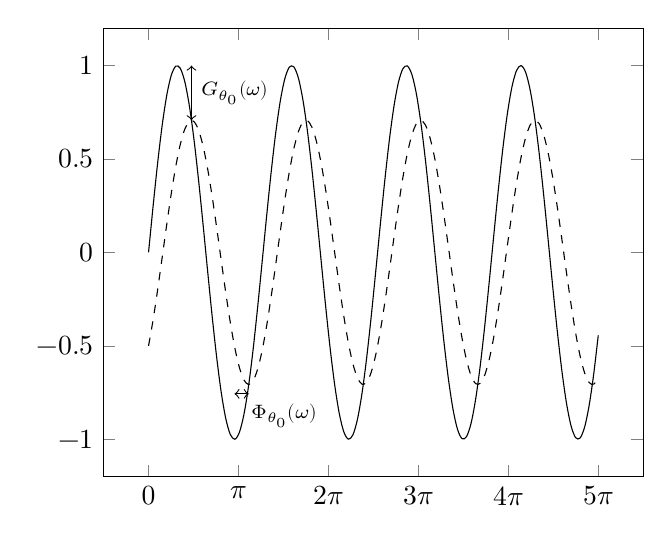
\begin{tikzpicture}
\begin{axis}[
xtick={0,3.14159,...,15.70795},
xticklabels={0,$\pi$,$2\pi$,$3\pi$,$4\pi$,$5\pi$}
]
\addplot[domain=0:5*pi,smooth]    plot (\x,{sin(\x * (pi/2) r)});
\addplot[domain=0:5*pi,smooth, dashed]
  plot (\x,{1/2*sin(\x* pi/2 r )+1/2*sin((\x -1) * pi/2 r)});
\draw[<->](axis cs: 1.5,1)--(axis cs: 1.5,0.7071068)
  node[pos=0.5, right]{\scriptsize $G_{\theta_0}(\omega)$};
\only<2->{
\draw[<->] (axis cs: 3, -0.70710680-0.05)--(axis cs: 3.5,-0.7071068-0.05)
  node[pos=0.5, below right]{\scriptsize $\Phi_{\theta_0}(\omega)$};}
\end{axis}
\end{tikzpicture}
\end{figure}
\end{frame}

\begin{frame}{Estimations de la TC et moyennes mobiles (2)}
\protect\hypertarget{estimations-de-la-tc-et-moyennes-mobiles-2}{}
\faArrowCircleRight{} Généralement, utilisation de filtres
\highlight{symétriques} (\(p=f\) et \(\theta_{-i}=\theta_i\))

\[
M_\theta(X_t)=\sum_{k=-p}^{+p}\theta_kX_{t+k}, \quad\text{avec }\theta_{-i}=\theta_i
\]

\pause

\faArrowCircleRight{} Pour l'estimation en \highlightbf{temps réel},
utilisation de filtres \highlight{asymétriques} (\(f<p\)) \(\implies\)
révision et détection avec retard des points de retournement
(\highlight{déphasage})

\[
\text{ex : }M_\theta(X_t)=\sum_{k=-p}^{0}\theta_kX_{t+k}
\]

\pause

Solution classique : prolonger la série par prévision et utiliser filtre
symétrique \faArrowCircleRight{} revient à utiliser des filtres
asymétriques optimisés avec certains critères\\
\faArrowCircleRight{} sous-optimal pour séries très variables
\end{frame}

\begin{frame}{Illustration avec climats des affaires dans les matériels
de transport}
\protect\hypertarget{illustration-avec-climats-des-affaires-dans-les-matuxe9riels-de-transport}{}
\begin{center}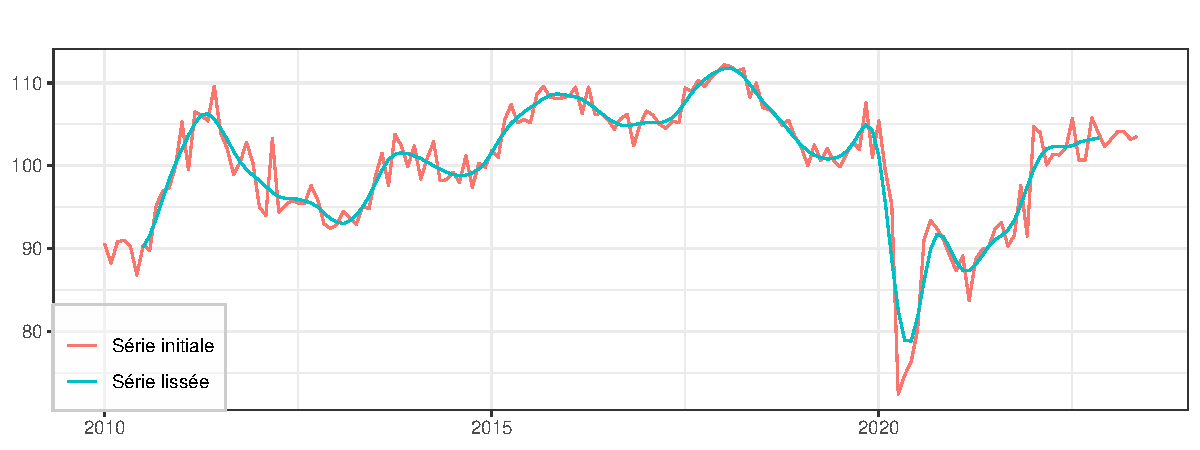
\includegraphics[width=1\linewidth]{img/ex/tc_finale} \end{center}
\footnotesize

\url{https://www.insee.fr/fr/statistiques/6522175}
\end{frame}

\begin{frame}[fragile]{Évaluer la qualité des estimations avec
prévisions implicites}
\protect\hypertarget{uxe9valuer-la-qualituxe9-des-estimations-avec-pruxe9visions-implicites}{}
Fonction \texttt{rjd3filters::implicit\_forecast}

\[
\forall q, \underbrace{\sum_{i=-h}^0 v_iy_i + \sum_{i=1}^h v_iy_i*}_{\text{lissage par }v\text{ de la série prolongée}}
=\underbrace{\sum_{i=-h}^0 w_i^qy_i + \sum_{i=1}^h w_i^qy_i*}_{\text{lissage par }w^q\text{ de la série prolongée}}\text{ avec }\forall i > q,w_i^q=0
\] Ce qui est équivalent à : \[
\forall q, \quad \sum_{i=1}^h (v_i- w_i^q) y_i^*
=\sum_{i=-h}^0 (w_i^q-v_i)y_i.
\] Matriciellement :

\begin{equation}
\resizebox{\textwidth}{!}{$
\begin{pmatrix}
  v_1 & v_2 & \cdots & v_h \\
  v_1 - w_1^1 & v_2 & \cdots & v_h \\
  \vdots & \vdots & \cdots & \vdots \\
   v_1 - w_1^{h-1} & v_2-w_2^{h-1} & \cdots & v_h
\end{pmatrix}
\begin{pmatrix}y_1^* \\ \vdots \\ y_h^*\end{pmatrix}=
\begin{pmatrix}
  w_{-h}^0 - v_{-h} & w_{-(h-1)}^0 - v_{-(h-1)} & \cdots & w_{0}^0 - v_{0} \\
  w_{-h}^1 - v_{-h} & w_{-(h-1)}^1 - v_{-(h-1)} & \cdots & w_{0}^1 - v_{0} \\
  \vdots & \vdots & \cdots & \vdots \\
  w_{-h}^{h-1} - v_{-h} & w_{-(h-1)}^{h-1} - v_{-(h-1)} & \cdots & w_{0}^{h-1} - v_{0}
\end{pmatrix}
\begin{pmatrix}y_{-h} \\ \vdots \\ y_0\end{pmatrix}.$}
\end{equation}
\end{frame}

\begin{frame}[fragile]{Objectifs}
\protect\hypertarget{objectifs}{}
Objectifs de cette étude :

\begin{itemize}
\item
  Étudier et comparer des approches récentes pour l'extraction de la
  tendance-cycle en temps réel : Régression polynomiale locale (Proietti
  et Luati 2008) ; RKHS (Dagum et Bianconcini 2016) ; Optimisation sous
  contrainte d'une somme pondérée de critères (Grun-Rehomme \emph{et
  ali} 2018, Wildi et McElroy, 2019)
\item
  On se concentre uniquement sur les moyennes mobiles asymétriques et
  pas sur l'estimation finale
\end{itemize}

\pause

\begin{itemize}
\item
  Montrer qu'il est possible d'établir une théorie générale englobant
  toutes ces méthodes et expliquer les liens entre les méthodes.
\item
  Permet d'avoir une revue de la littérature de l'existant.
\end{itemize}

\pause

\begin{itemize}
\tightlist
\item
  Présenter le package \faIcon{r-project} \texttt{rjd3filters}
  \url{https://github.com/rjdemetra/rjd3filters}
\end{itemize}
\end{frame}

\hypertarget{muxe9thodes-uxe9tudiuxe9es}{%
\section{Méthodes étudiées}\label{muxe9thodes-uxe9tudiuxe9es}}

\hypertarget{filtre-symuxe9trique}{%
\subsection{Filtre symétrique}\label{filtre-symuxe9trique}}

\begin{frame}[fragile]{Moyenne mobile symétrique d'Henderson}
\protect\hypertarget{moyenne-mobile-symuxe9trique-dhenderson}{}
\begin{columns}[T]
\begin{column}{0.55\textwidth}
\footnotesize

\begin{Shaded}
\begin{Highlighting}[]
\FunctionTok{library}\NormalTok{(rjd3filters)}
\NormalTok{f }\OtherTok{\textless{}{-}} \FunctionTok{lp\_filter}\NormalTok{(}\DecValTok{6}\NormalTok{, }\AttributeTok{kernel =} \StringTok{"Henderson"}\NormalTok{)}
\FunctionTok{plot\_coef}\NormalTok{(f, }\AttributeTok{q =} \DecValTok{6}\NormalTok{, }\AttributeTok{legend =} \ConstantTok{FALSE}\NormalTok{,}
          \AttributeTok{main=}\StringTok{"Henderson 13 termes"}\NormalTok{)}
\end{Highlighting}
\end{Shaded}

\begin{center}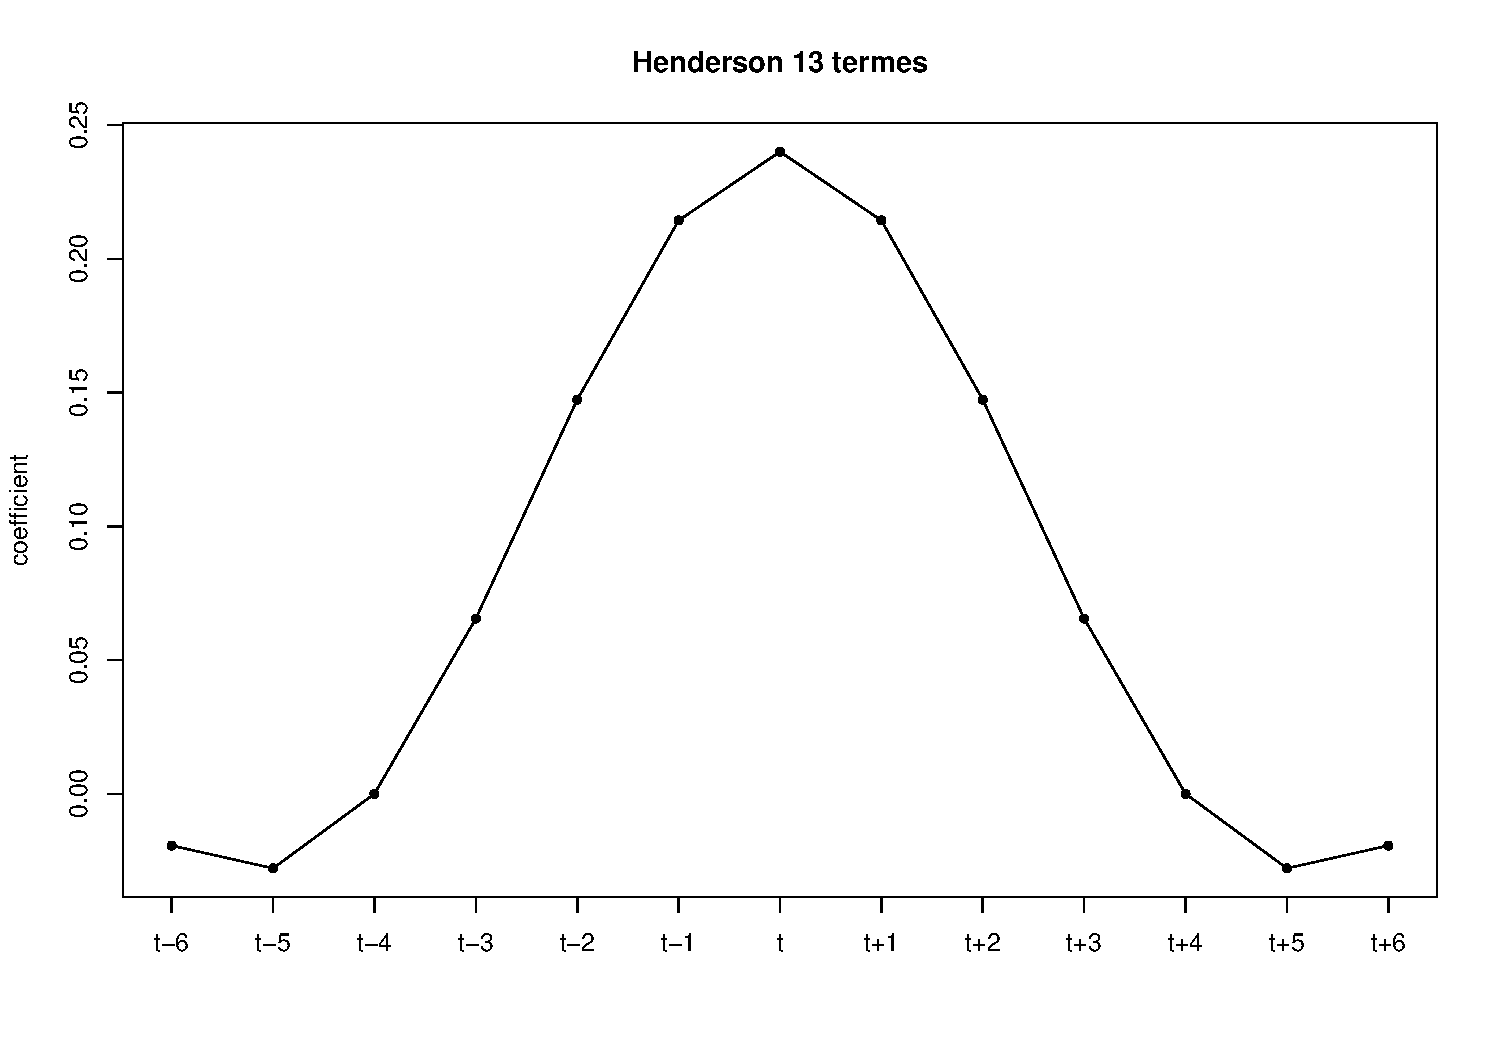
\includegraphics[height=0.4\paperheight]{img/rmd-h13-1} \end{center}
\end{column}

\begin{column}{0.45\textwidth}
MM Henderson (utilisé dans X-13ARIMA) largement répandue pour estimer
\(TC_t\)

\medskip

MM Henderson préserve les tendances polynomiales de degré 3 et minimise
le critère de ``lissage'' (\(\sum(\nabla^3\theta_i)^2\))

\medskip

Sur séries mensuelles : MM de 13 termes généralement
\end{column}
\end{columns}
\end{frame}

\hypertarget{polynuxf4mes-locaux}{%
\subsection{Polynômes Locaux}\label{polynuxf4mes-locaux}}

\begin{frame}{Polynômes Locaux : \texttt{rjd3filters::lp\_filter()}}
\protect\hypertarget{polynuxf4mes-locaux-rjd3filterslp_filter}{}
Hypothèse : \(y_t=\mu_t+\varepsilon_t\) avec
\(\varepsilon_t\overset{i.i.d}{\sim}\mathcal N(0,\sigma^2)\)

\(\mu_t\) localement approchée par un polynôme de degré \(d\): \[
\forall j\in\left\llbracket -h,h\right\rrbracket : y_{t+j}=m_{t+j}+\varepsilon_{t+j},\quad m_{t+j}=\sum_{i=0}^{d}\beta_{i}j^{i}
\]

\pause

Estimation en utilisant les WLS avec \emph{noyaux}:
\(\hat{\beta}=(X'KX)^{1}X'Ky\) et \[
\hat{m}_{t}=\hat\beta_0=w'y=\sum_{j=-h}^{h}w_{j}y_{t-j}
\text{ \faArrowCircleRight{} équivalent à une moyenne mobile symétrique}
\] \faArrowCircleRight{} Filtre de Henderson avec \(d=3\) et noyau
spécifique.
\end{frame}

\begin{frame}[fragile]{Filtres asymétriques :
\texttt{rjd3filters::lp\_filter()}}
\protect\hypertarget{filtres-asymuxe9triques-rjd3filterslp_filter}{}
\begin{enumerate}
\tightlist
\item
  Même méthode mais moins de données (DAF) \(\iff\) minimiser les
  révisions sous mêmes contraintes polynomiales
\end{enumerate}

\faArrowCircleRight{} \textbf{sans biais} mais \textbf{beaucoup de
variance}

\faArrowCircleRight{} utilisé dans STL

\pause

\begin{enumerate}
\setcounter{enumi}{1}
\item
  Minimisation des révisions sous contraintes polynomiales :

  \begin{enumerate}
  \item
    \emph{Linear-Constant} (LC): \(y_t\) linéaire and \(v\) reproduit
    les constantes (\highlight{Musgrave})
  \item
    \emph{Quadratic-Linear} (QL): \(y_t\) quadratique et \(v\) reproduit
    droites
  \item
    \emph{Cubic-Quadratic} (CQ): \(y_t\) cubique et \(v\) reproduit
    tendances quadratiques
  \end{enumerate}

  \faArrowCircleRight{} Filtres asymétriques \(v\) dépendent de
  ``IC-Ratio''
\end{enumerate}

\pause

\bcsmbh modèles simples facilement interprétables

\bcsmmh Déphasage non contrôlé \faArrowCircleRight{} méthode étendue
dans \texttt{rjd3filters::lp\_filter()}

\pause

\faDesktop{} Visualisation
\url{https://aqlt.shinyapps.io/FiltersProperties/}
\end{frame}

\begin{frame}{Coefficients}
\protect\hypertarget{coefficients}{}
\begin{center}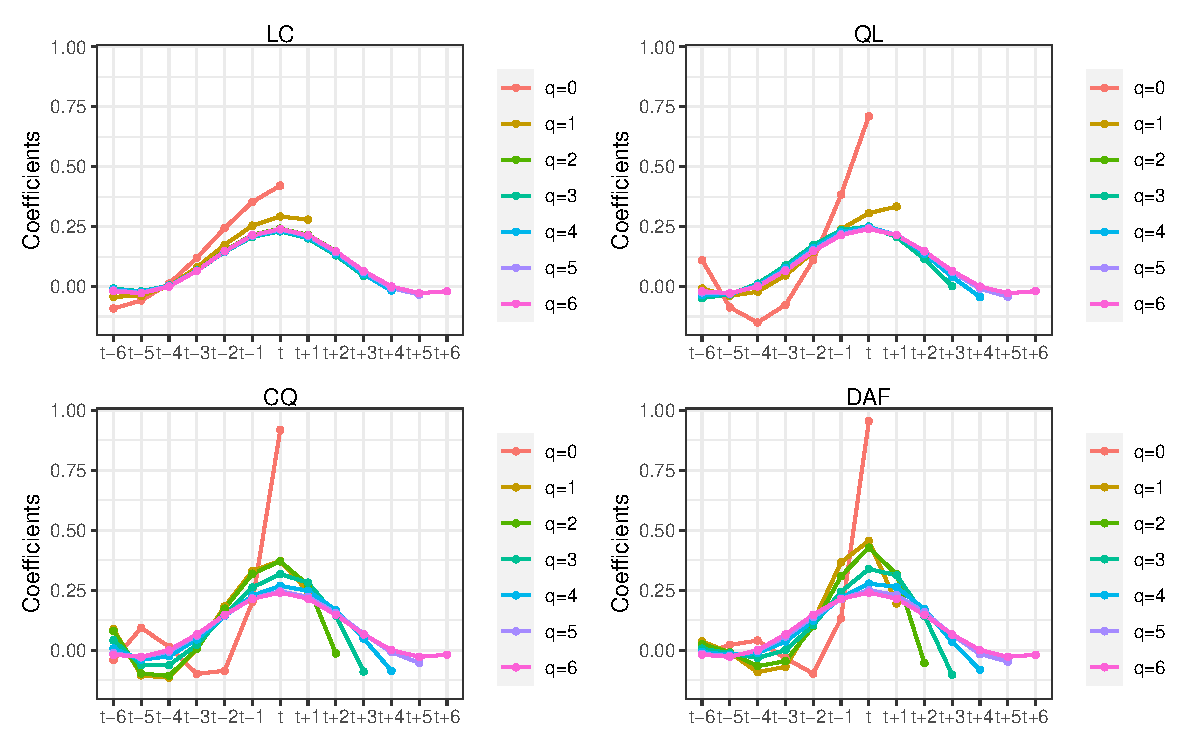
\includegraphics[height=0.9\textheight]{img/coefs_lp} \end{center}
\end{frame}

\begin{frame}{Illustration (1)}
\protect\hypertarget{illustration-1}{}
\begin{center}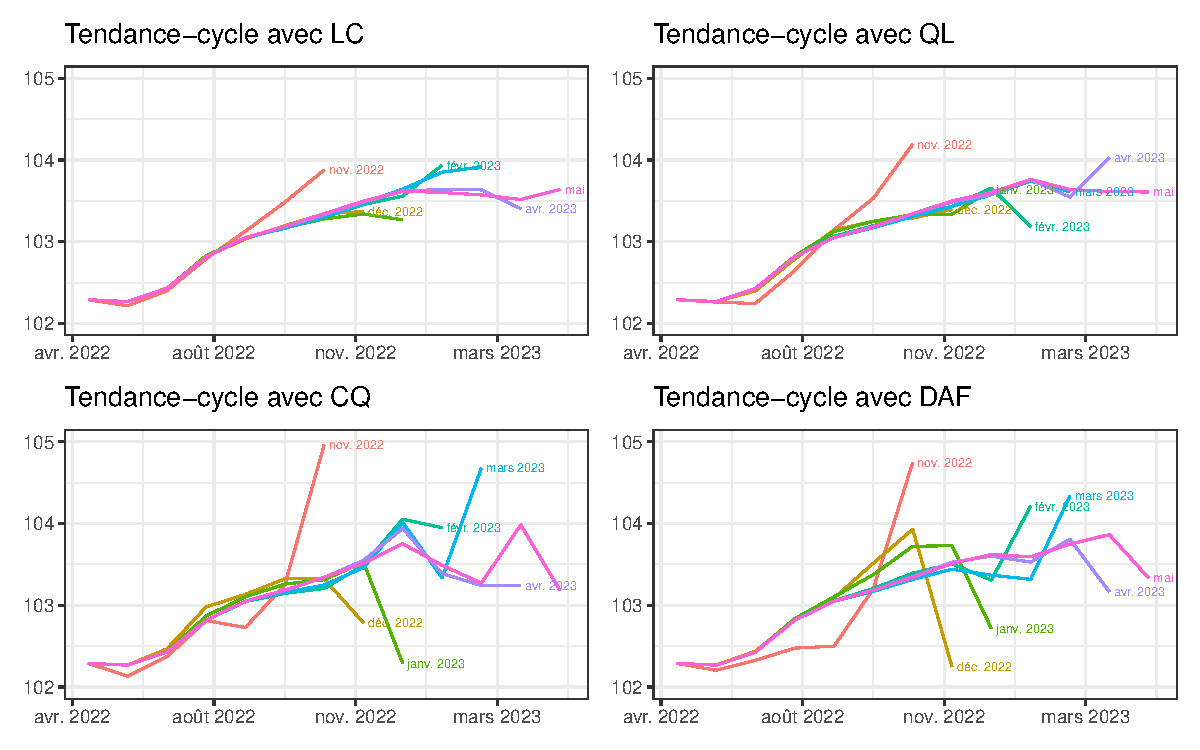
\includegraphics[width=1\linewidth]{img/ex/lp_es} \end{center}
\end{frame}

\begin{frame}{Illustration (2)}
\protect\hypertarget{illustration-2}{}
\begin{center}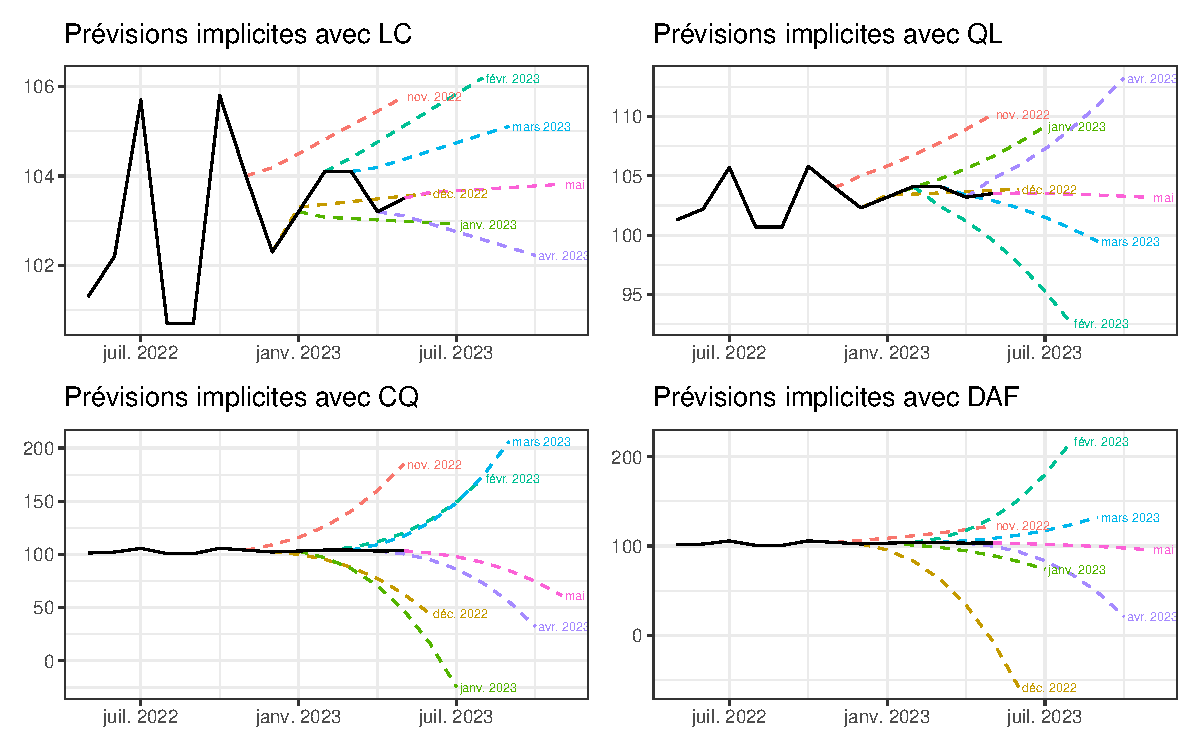
\includegraphics[width=1\linewidth]{img/ex/lp_if} \end{center}
\end{frame}

\hypertarget{filtres-et-reproducing-kernel-hilbert-space-rkhs}{%
\subsection{Filtres et Reproducing Kernel Hilbert Space
(RKHS)}\label{filtres-et-reproducing-kernel-hilbert-space-rkhs}}

\begin{frame}{Filtres RKHS : \texttt{rjd3filters::rkhs\_filter()}}
\protect\hypertarget{filtres-rkhs-rjd3filtersrkhs_filter}{}
\begin{itemize}
\item
  Utilisation de la théorie des RKHS pour approcher le filtre
  d'Henderson
\item
  Avec \(K_p\) une \textbf{fonction de noyau} définie sur \([-1,1]\), le
  filtre symétrique : \[
  \forall j\in\left\llbracket -h,h\right\rrbracket: w_{j}=\frac{K_p(j/b)}{\sum_{i=-h}^{^h}K_p(i/b)}
  \]
\end{itemize}

\onslide<3->{\faArrowCircleRight{} avec $b=h+1$ et $K_p$ spécifique on retrouve le filtre d'Henderson}

\pause

\begin{itemize}
\tightlist
\item
  Pour les filtres asymétriques : \[
  \forall j\in\left\llbracket -h,q\right\rrbracket: w_{a,j}=\frac{K_p(j/b)}{\sum_{i=-h}^{^q}K_p(i/b)}
  \]
\end{itemize}

\pause\pause\faArrowCircleRight{} \(b\) choisit par optimisation,
e.g.~minimisant les révisions (\(b_{q,\Gamma}\)), les révisions liées à
la fonction de gain (\(b_{q,G}\)) et celles liées au déphasage
(\(b_{q,\varphi}\))
\end{frame}

\begin{frame}[fragile]{Filtres asymétriques}
\protect\hypertarget{filtres-asymuxe9triques}{}
\begin{columns}[T]
\begin{column}{0.65\textwidth}
\bcsmmh Plusieurs extremum

\footnotesize

\begin{Shaded}
\begin{Highlighting}[]
\FunctionTok{library}\NormalTok{(rjd3filters)}
\NormalTok{fun }\OtherTok{\textless{}{-}} \FunctionTok{rkhs\_optimization\_fun}\NormalTok{(}\AttributeTok{horizon =} \DecValTok{6}\NormalTok{,}
            \AttributeTok{leads =} \DecValTok{5}\NormalTok{, }\AttributeTok{degree =} \DecValTok{3}\NormalTok{,}
            \AttributeTok{asymmetricCriterion =} \StringTok{"Timeliness"}\NormalTok{)}
\FunctionTok{plot}\NormalTok{(fun, }\FloatTok{5.6}\NormalTok{, }\DecValTok{12}\NormalTok{, }\AttributeTok{xlab =} \StringTok{"b"}\NormalTok{,}
     \AttributeTok{ylab =} \StringTok{"Timeliness"}\NormalTok{, }\AttributeTok{main =} \StringTok{"6X5 filter"}\NormalTok{)}
\end{Highlighting}
\end{Shaded}

\begin{center}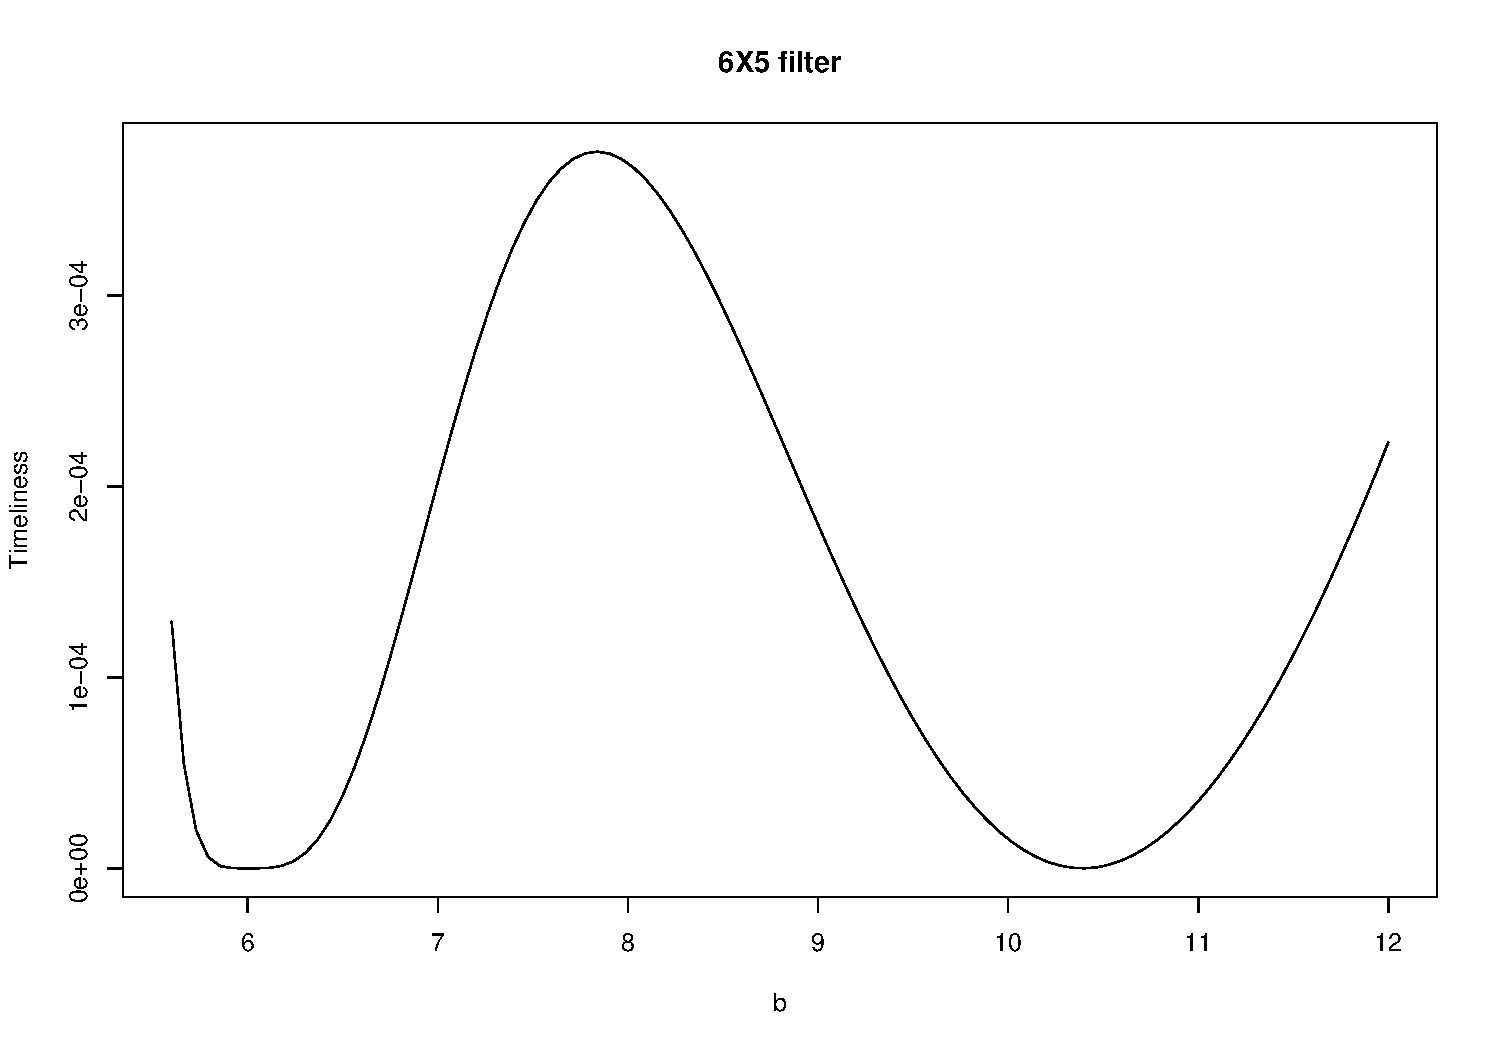
\includegraphics[height=0.4\paperheight]{img/rmd-rkhstimeliness-1} \end{center}

\begin{Shaded}
\begin{Highlighting}[]
\FunctionTok{rkhs\_optimal\_bw}\NormalTok{()}
\end{Highlighting}
\end{Shaded}

\begin{verbatim}
##    q=0    q=1    q=2    q=3    q=4    q=5 
## 6.0000 6.0000 6.3875 8.1500 9.3500 6.0000
\end{verbatim}
\end{column}

\begin{column}{0.3\textwidth}
\bigskip

\bcsmbh Méthode généralisable à des filtres avec fréquences irrégulières
\end{column}
\end{columns}
\end{frame}

\begin{frame}{Coefficients}
\protect\hypertarget{coefficients-1}{}
\begin{center}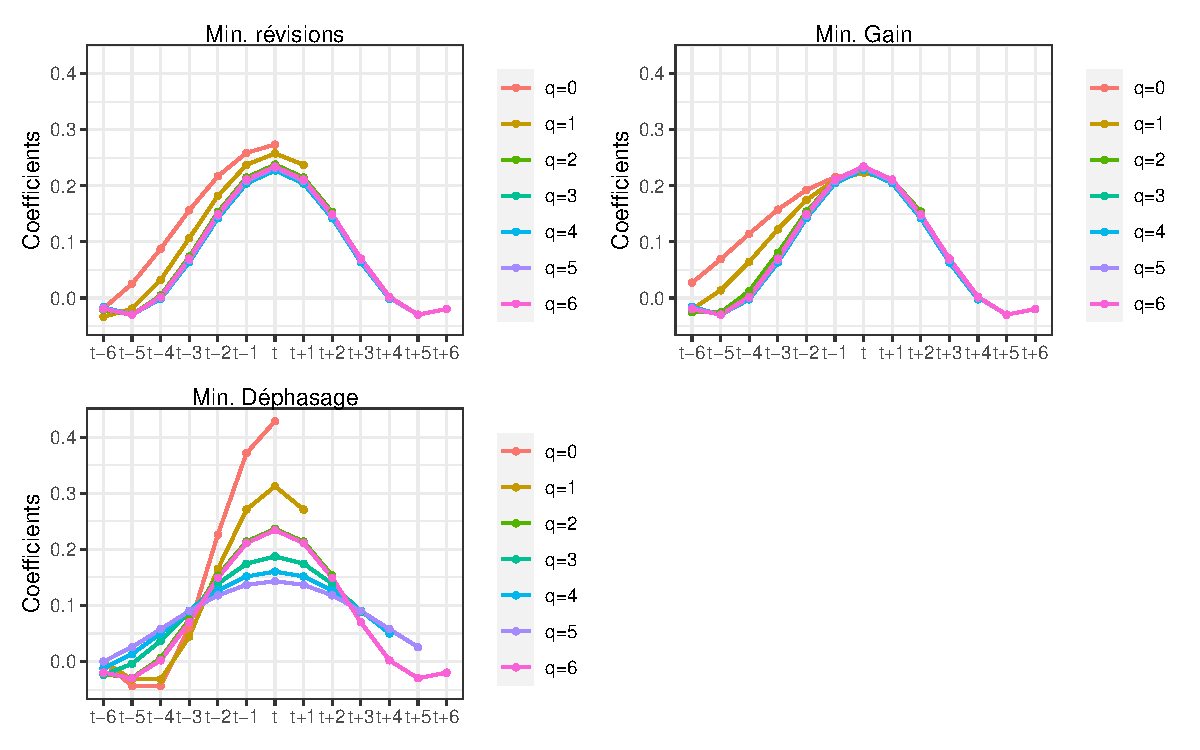
\includegraphics[height=0.9\textheight]{img/coefs_rkhs} \end{center}
\end{frame}

\begin{frame}{Illustration (1)}
\protect\hypertarget{illustration-1-1}{}
\begin{center}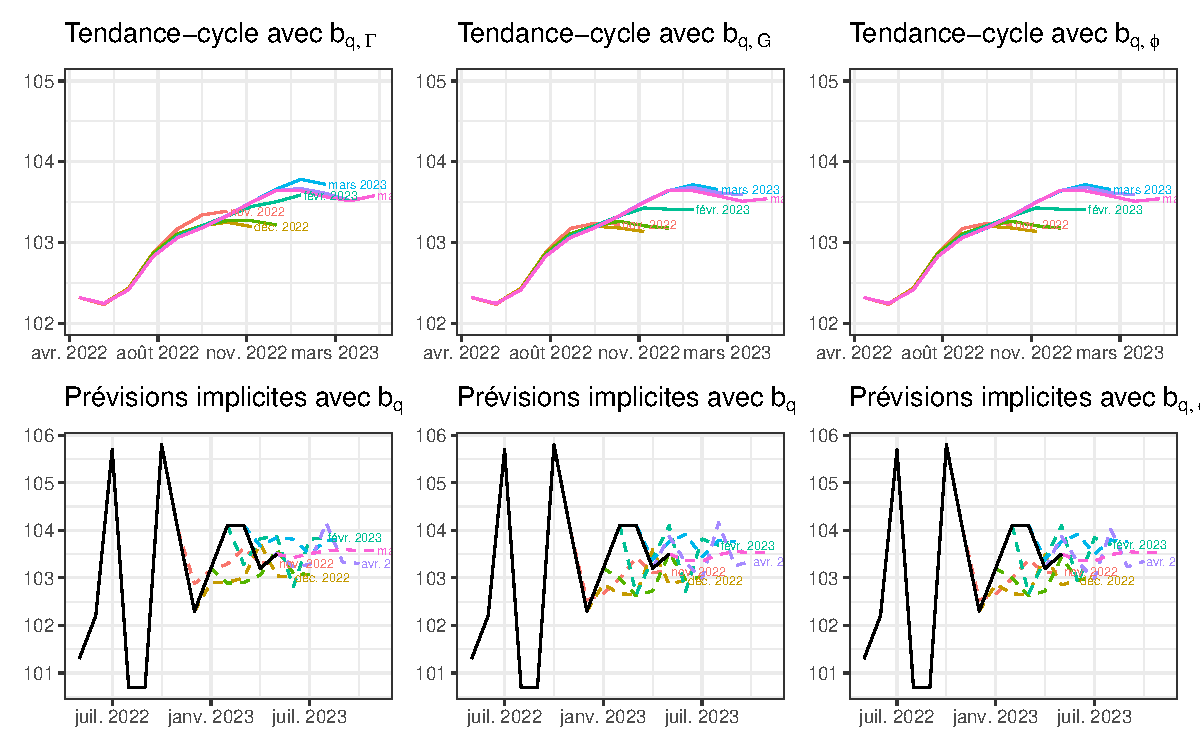
\includegraphics[width=1\linewidth]{img/ex/rkhs} \end{center}
\end{frame}

\hypertarget{minimisation-sous-contrainte-fst-et-ats}{%
\subsection{Minimisation sous contrainte : FST et
ATS}\label{minimisation-sous-contrainte-fst-et-ats}}

\begin{frame}{Approche FST : \texttt{rjd3filters::fst\_filter()}}
\protect\hypertarget{approche-fst-rjd3filtersfst_filter}{}
Minimisation sous contrainte d'une somme pondérée de 3 critères :

\[
\begin{cases}
\underset{\theta}{\min} & J(\theta)=
\alpha F_g(\theta)+\beta S_g(\theta)+\gamma T_g(\theta)\\
s.c. & C\theta=a
\end{cases}
\] \(F_g\) fidélité (\emph{fidelity}, réduction de variance
\(\sum_{k=-p}^{+f} \theta_k^2\)), \(S_g\) lissage (\emph{smoothness},
critère d'Henderson \(\sum_{j}(\nabla^{3}\theta_{j})^{2}\)), \(T_g\)
temporalité (\emph{timeliness}, déphasage
\(\int_{0}^{2\pi/12}\rho_{\theta}(\omega)\sin(\varphi_{\theta}(\omega))^{2}\ud\omega\))

\pause

\begin{summary}

\begin{itemize}
\item
  \bcsmbh Solution unique
\item
  \bcsmbh Filtres asymétriques indépendants des données et du filtre
  symétrique
\item
  \bcsmmh Poids non normalisés
\end{itemize}

\end{summary}
\end{frame}

\begin{frame}{Illustration (1)}
\protect\hypertarget{illustration-1-2}{}
\begin{center}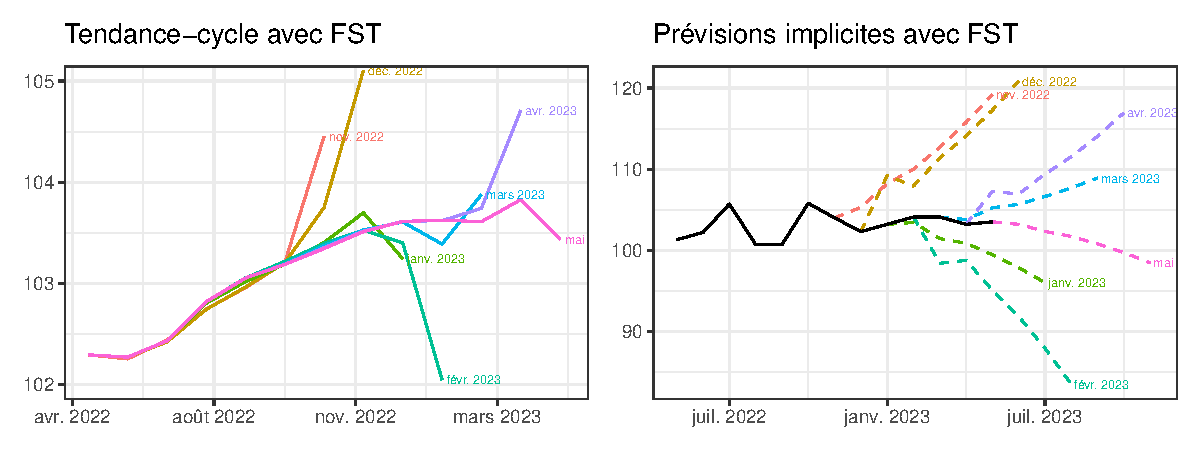
\includegraphics[width=1\linewidth]{img/ex/fst} \end{center}
\end{frame}

\begin{frame}[allowframebreaks]{Approche ATS
\texttt{rjd3filters::dfa\_filter()}}
\protect\hypertarget{approche-ats-rjd3filtersdfa_filter}{}
Décomposition de l'EQM : \begin{align*}
&\E{(y_{t}-\hat{y}_{t})^{2}}=\frac{1}{2\pi}\int_{-\pi}^{\pi}\left|\Gamma_s(\omega)-{\Gamma_\theta}(\omega)\right|^{2}h(\omega)\ud\omega \nonumber
\\&\quad=\frac{1}{2\pi}\times2\times\int_{0}^{\pi}\left|\Gamma_s(\omega)-{\Gamma_\theta}(\omega)\right|^{2}h(\omega)\ud\omega
\end{align*} et \begin{align*}
&\left|\Gamma_s(\omega)-\Gamma_\theta(\omega)\right|^{2}=\rho_s(\omega)^{2}+\rho_\theta(\omega)^{2} + \\
&\qquad \phantom{=}2\rho_s(\lambda)\rho_\theta(\lambda)\left(1-\cos(\varphi_s(\omega)-\varphi_\theta(\omega)\right) \\
 &\qquad =\left(\rho_s(\omega)-\rho_\theta(\omega)\right)^{2}+\\
&\qquad \phantom{=}4\rho_s(\lambda)\rho_\theta(\lambda)\sin^{2}\left(\frac{\varphi_s(\omega)-\varphi_\theta(\omega)}{2}\right)
\end{align*}

Ce qui conduit à \begin{align*}
A_w&= 2\int_0^{\omega_1}\left(\rho_s(\omega)-\rho_\theta(\omega)\right)^{2}h(\omega)\ud\omega\\
T_w&= 8\int_0^{\omega_1}\rho_s(\lambda)\rho_\theta(\lambda)\sin^{2}\left(\frac{\varphi_\theta(\omega)}{2}\right)h(\omega)\ud\omega\\
S_w&= 2\int_{\omega_1}^\pi\left(\rho_s(\omega)^{2}-\rho_\theta(\omega)\right)^{2}h(\omega)\ud\omega\\
R_w&= 8\int_{\omega_1}^\pi\rho_s(\lambda)\rho_\theta(\lambda)\sin^{2}\left(\frac{\varphi_\theta(\omega)}{2}\right)h(\omega)\ud\omega\\
\end{align*}

Minimisation d'une somme pondérée de 3 critères : \[
\mathcal{M}(\vartheta_{1},\vartheta_{2})=\vartheta_{1}T_w(\theta)+\vartheta_{2}S_w(\theta)+(1-\vartheta_{1}-\vartheta_{2})A_w(\theta)
\] \(\implies\) minimisation sous contraintes linéaires avec
\(h(\omega)=1\)

\begin{summary}

\begin{itemize}
\item
  \bcsmbh Poids ont un sens
\item
  \bcsmmh Résidus pas toujours négligeables
\item
  \bcsmmh Pas unicité de la solution
\end{itemize}

\end{summary}
\end{frame}

\begin{frame}{Difficulté du choix des poids}
\protect\hypertarget{difficultuxe9-du-choix-des-poids}{}
Comment choisir les poids dans FST et AST (DFA) ?

\begin{itemize}[<+->]
\item
  Minimiser que la \emph{timeliness} ? introduit trop de variance
\item
  Minimiser les révisions ? on néglige le déphasage
\item
  Faire quadrillage du plan et une analyse empirique du déphasage ?
  C'est ce qui est fait avec FST en prenant les poids qui minimisent le
  déphasage sur les séries simulées (avec différents niveaux de
  variabilité). Toujours du filtre préservant les polynômes de degré 2
  avec \(\alpha\)=0,00 (fidelity), \(\beta\)=0,05 (smoothness) et
  \(\gamma\)=0,95 (timeliness).
\end{itemize}
\end{frame}

\hypertarget{extensions}{%
\section{Extensions}\label{extensions}}

\hypertarget{choix-de-la-fenuxeatre}{%
\subsection{Choix de la fenêtre}\label{choix-de-la-fenuxeatre}}

\begin{frame}[allowframebreaks]{Combien de termes utiliser les MM
asymétriques ?}
\protect\hypertarget{combien-de-termes-utiliser-les-mm-asymuxe9triques}{}
Actuellement on utilise toujours autant de points dans le passé (6) que
la MM symétriques pour les estimations intermédiaires : hypothèse
raisonnable ? Faudrait-il utiliser plus ou moins de points dans le passé
?

Critères classiques : validation croisée, CP-Mallow, AIC, Rice-T :

\[
CV(\hat\mu)=\frac{1}{n-2h}\sum_{t=h+1}^{n-h}\frac{(y_t-\hat \mu_t)^2}{(1-w_0)^2}
\] \[
CP(\hat\mu)=\frac{1}{\sigma^2}\sum_{t=h+1}^{n-h}(y_t-\hat \mu_t)^2 - (n-2h)(1-2w_0)
\] Mais en général leur minimisation ne donne pas de bon résultats
(critères peu discriminants)

Pistes à explorer :

\begin{enumerate}
\item
  Méthodes plus complexes de sélection de la fenêtre (e.g.~Fan et
  Gijbels 1992)
\item
  Méthode des plus proches voisins : utiliser toujours le même nombre de
  points (e.g.~toujours 13 points)
\end{enumerate}
\end{frame}

\hypertarget{paramuxe9trisation-locale-des-muxe9thodes-polynomiales}{%
\subsection{Paramétrisation locale des méthodes
polynomiales}\label{paramuxe9trisation-locale-des-muxe9thodes-polynomiales}}

\begin{frame}[allowframebreaks]{Estimation de la pente}
\protect\hypertarget{estimation-de-la-pente}{}
Régression non paramétrique : \(y_i=\mu(x_i)+\varepsilon_i\) avec
\(\varepsilon_i\) un terme d'erreur.

Avec Taylor, pour tout point \(x_0\), si \(\mu\) est différentiable
\(d\) fois, alors : \[
\forall x \::\:\mu(x) = \mu(x_0) + \mu'(x_0)(x-x_0)+\dots +
\frac{\mu^{(d)}(x_0)}{d!}(x-a)^d+R_d(x),
\]

Régression polynomiale

Hypothèse : \(y_t=\mu_t+\varepsilon_t\) avec
\(\varepsilon_t\overset{i.i.d}{\sim}\mathcal N(0,\sigma^2)\)

\(\mu_t\) localement approchée par un polynôme de degré \(d\): \[
\forall j\in\left\llbracket -h,h\right\rrbracket : y_{t+j}=\sum_{i=0}^{d}\beta_{i}j^{i}+\varepsilon_{t+j}
\]

Estimation en utilisant les WLS avec \emph{noyaux} :
\(\hat{\beta}=(X'KX)^{1}X'Ky\) et \[
\hat{m}_{t}=\hat\beta_0=e_1'\hat{\beta} =w'y=\sum_{j=-h}^{h}w_{j}y_{t-j}\text{ avec }
e_1=\begin{pmatrix}1\\ 0\\\vdots\\0\end{pmatrix}
\] Et de la même façon : \[
\begin{cases}
\hat\beta_1 = \widehat{\mu'(t)}= e_2'\hat{\beta}\qquad(\ne \widehat{\mu(t)}') \\
\hat\beta_2 = \widehat{\mu''(t)}= e_3'\hat{\beta}
\end{cases}
\]

Dans la méthode LC, en fin de période on suppose : \[
y_t=\beta_0+\beta_1t+\varepsilon_t\text{ avec }\varepsilon_t\sim\mathcal N (0,\sigma^2)
\] Filtres asymétriques dépendent du ratio \(|\beta_1/\sigma|\) qui est
toujours supposé constant : peu de sens au niveau global, notamment dans
les périodes de points de retournement (\(\beta_1\simeq 0\))

\begin{center}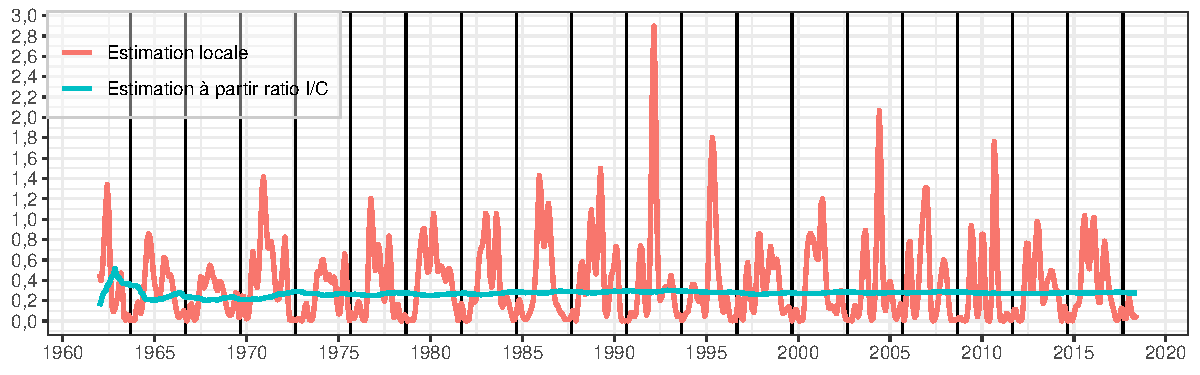
\includegraphics[width=1\linewidth]{img/local_ic_tp} \end{center}

Idée : paramétrisation locale \[
\begin{cases}
\hat\sigma^2=\frac{1}{n-2h}\sum_{t=h+1}^{n-h}\frac{(y_t-\hat \mu_t)^2}{1-2w_0^2+\sum w_i^2}\\
\beta_1\text{ et }\beta_2 \text{ estimés par MM (DAF par simplification)}
\end{cases}
\]

\begin{center}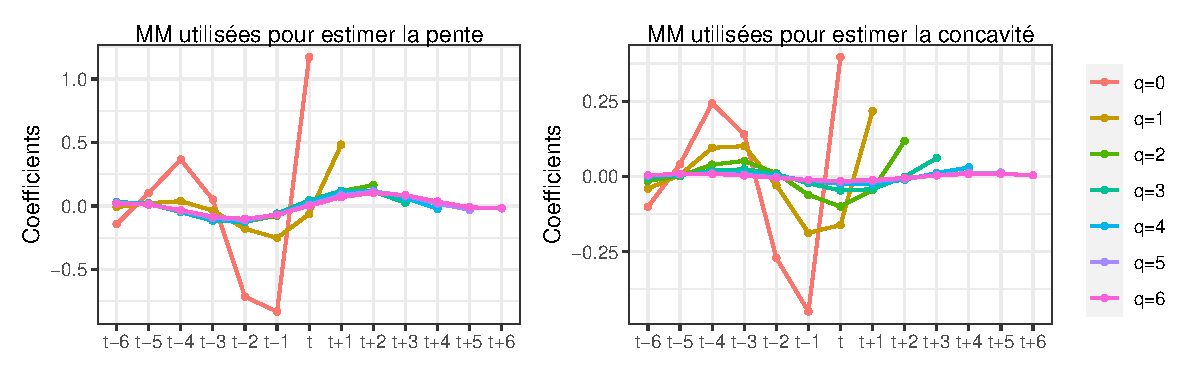
\includegraphics[width=1\linewidth]{img/local_ic_mm} \end{center}

Rmq: il y a (encore) de fortes révisions entre la première et deuxième
estimation, on pourrait utiliser méthode QL pour avoir les estimateurs
de la pente

Spoil : marche plutôt bien
\end{frame}

\begin{frame}{Illustration (1)}
\protect\hypertarget{illustration-1-3}{}
\begin{center}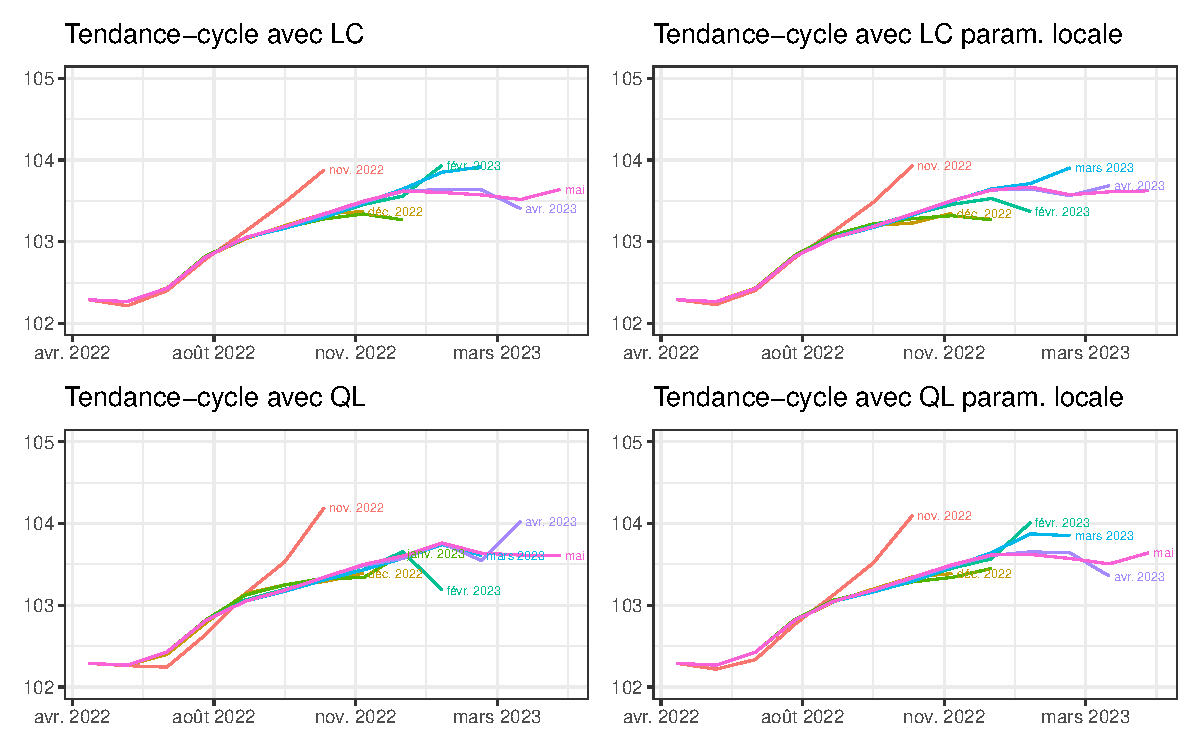
\includegraphics[width=1\linewidth]{img/ex/lp_local_es} \end{center}
\end{frame}

\begin{frame}{Illustration (2)}
\protect\hypertarget{illustration-2-1}{}
\begin{center}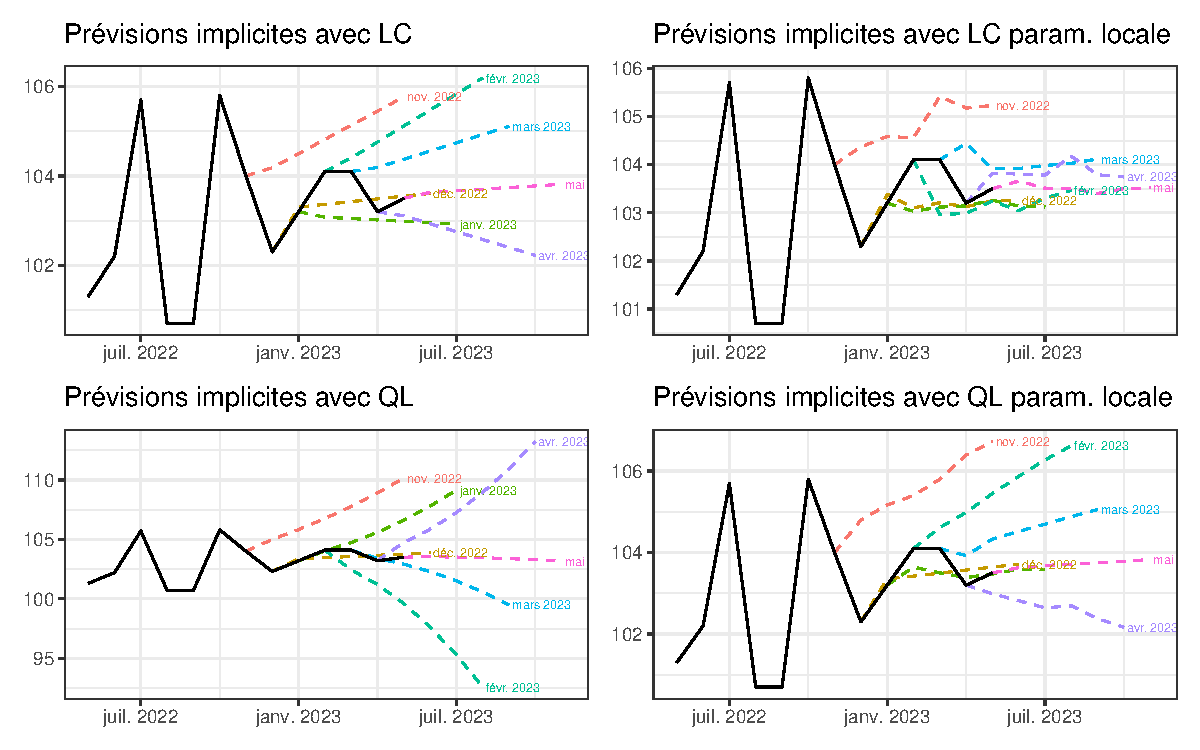
\includegraphics[width=1\linewidth]{img/ex/lp_local_if} \end{center}
\end{frame}

\hypertarget{comparaison-des-muxe9thodes}{%
\section{Comparaison des méthodes}\label{comparaison-des-muxe9thodes}}

\hypertarget{muxe9thodologie}{%
\subsection{Méthodologie}\label{muxe9thodologie}}

\begin{frame}{Méthodologie}
\protect\hypertarget{muxe9thodologie-1}{}
Comparaison des différentes méthodes sur séries simulées (avec 3 niveaux
de variabilité) et séries réelles :

\begin{enumerate}
\tightlist
\item
  Estimation de la tendance-cycle à chaque date en utilisant les
  différentes méthodes et un filtre symétrique de 13 termes
\end{enumerate}

\pause

\begin{enumerate}
\setcounter{enumi}{1}
\item
  À chaque date, estimation des points de retournement :

  \begin{itemize}
  \item
    redressements : \(y_{t-3}\geq y_{t-2}\geq y_{t-1}<y_t\leq y_{t+1}\)
  \item
    ralentissements :
    \(y_{t-3}\leq y_{t-2}\leq y_{t-1}>y_t\geq y_{t+1}\)
  \end{itemize}
\end{enumerate}

Déphasage = temps nécessaire pour détecter le bon point de retournement
\highlight{sans révision} (\(\ne\) des papiers classiques)

\pause

\begin{enumerate}
\setcounter{enumi}{2}
\tightlist
\item
  Calcul des révisions avec deux critères :
\end{enumerate}

\[
\mathbb E\left[
\left|\frac{
y_{t|t+q} - y_{t|last}
}{
y_{t|last}
}\right|
\right]\quad
\text{ et }
\quad
\mathbb E\left[
\left|\frac{
y_{t|t+q} - y_{t|t+q+1}
}{
y_{t|t+q+1}
}\right|
\right]
\]
\end{frame}

\begin{frame}[allowframebreaks]{Séries simulées}
\protect\hypertarget{suxe9ries-simuluxe9es}{}
De façon similaire à Darne et Dagum (2009), on simule
\(y_t= C_t+ T_t + I_t\) entre janvier 1960 et décembre 2020 :

\begin{itemize}
\item
  \(C_t = \rho [\cos (2 \pi t / \lambda) +\sin (2 \pi t / \lambda)]\),
  \(\lambda=72\) (cycles de 6 ans, 19 points de retournement
  détectables)
\item
  \(T_t = T_{t-1} + \nu_t\) avec
  \(\nu_t \sim \mathcal{N}(0, \sigma_\nu^2)\), \(\sigma_\nu=0,08\)
\item
  \(I_t = e_t\) avec \(e_t \sim \mathcal{N}(0, \sigma_e^2)\)
\end{itemize}

Niveau de variabilité :

\begin{itemize}
\item
  variabilité faible (rapport signal/bruit fort) : \(\sigma_e^2=0,2\) et
  \(\rho = 3,0,\, 3,5\) ou \(4,0\) (0,9 \(\geq\) I-C ratio \(\geq\) 0,7)
\item
  variabilité moyenne (rapport signal/bruit moyen) : \(\sigma_e^2=0,3\)
  et \(\rho = 1,5,\, 2,0\) ou \(3,0\) (2,3 \(\geq\) I-C ratio \(\geq\)
  1,4)
\item
  variabilité forte (rapport signal/bruit élevé) : \(\sigma_e^2=0,4\) et
  \(\rho = 0,5,\, 0,7\) ou \(1,0\) (8,9 \(\geq\) I-C ratio \(\geq\) 5,2)
\end{itemize}

\begin{center}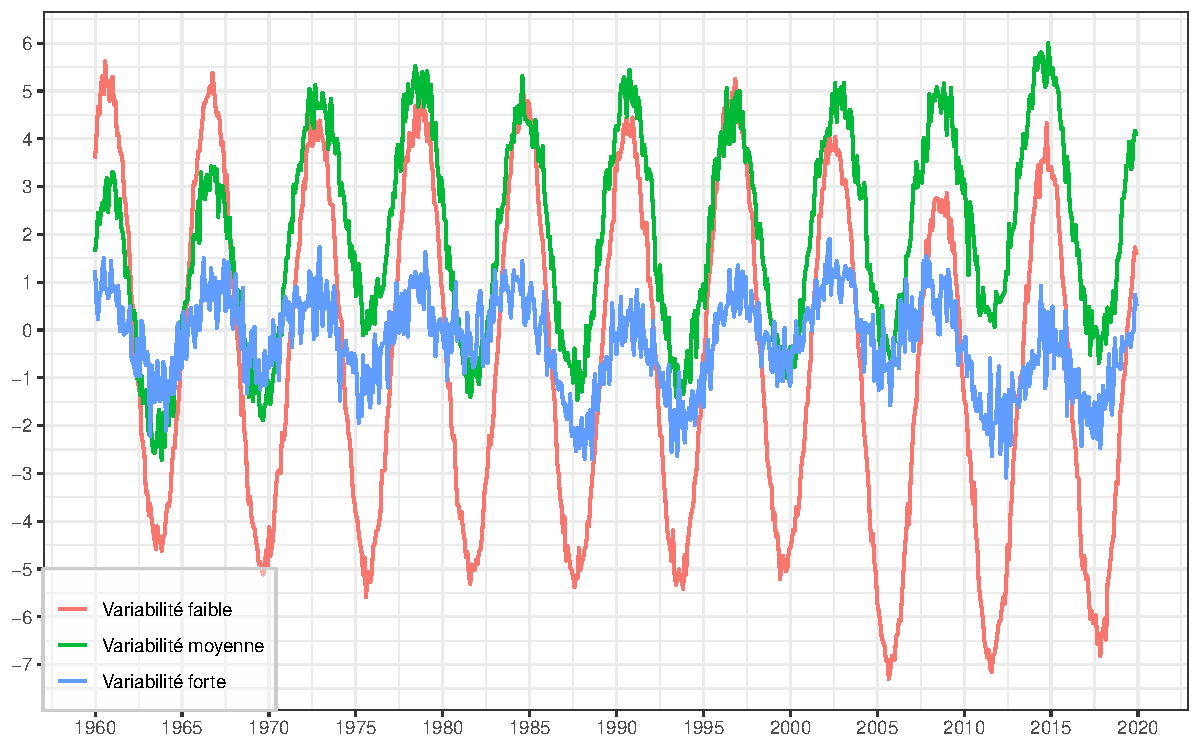
\includegraphics[width=1\linewidth]{img/simul_data} \end{center}
\end{frame}

\hypertarget{application}{%
\subsection{Application}\label{application}}

\begin{frame}{Résultats sur séries simulées}
\protect\hypertarget{ruxe9sultats-sur-suxe9ries-simuluxe9es}{}
Voir
\url{https://aqlt.github.io/DT-est-tr-tc/sec-comparison.html\#comparaison}
\end{frame}

\begin{frame}{Résultats sur des séries réelles}
\protect\hypertarget{ruxe9sultats-sur-des-suxe9ries-ruxe9elles}{}
Voir
\url{https://aqlt.github.io/DT-est-tr-tc/sec-comparison.html\#s\%C3\%A9rie-r\%C3\%A9elle}
\end{frame}

\begin{frame}[fragile]{Nouvelle Bibliographique}
\protect\hypertarget{nouvelle-bibliographique}{}
Estela Bee Dagum \& Silvia Bianconcini (June 2023): Monitoring the
direction of the short-term trend of economic indicators

\begin{itemize}
\item
  étudient le filtre cascade avec une approximation via les RKHS en
  utilisant noyau triangulaire (coefficients non retrouvé avec
  \texttt{rjd3filters})
\item
  proposent deux tests statistiques pour comparer les méthodes en termes
  de révisions et de point de retournement
\item
  Comparent les méthodes en étudiant deux séries de la FRED
\end{itemize}
\end{frame}

\hypertarget{conclusion}{%
\section{Conclusion}\label{conclusion}}

\hypertarget{conclusion-1}{%
\subsection{Conclusion}\label{conclusion-1}}

\begin{frame}[fragile]{Conclusion}
\protect\hypertarget{conclusion-2}{}
\begin{itemize}
\tightlist
\item
  Dans la construction des filtres asymétriques:
\end{itemize}

\begin{enumerate}
\tightlist
\item
  on peut se restreindre à ceux qui conservent les polynômes de degré au
  plus 1 (et exclure les filtres QL, CQ et DAF)
\end{enumerate}

\bigskip

\pause

\begin{enumerate}
\setcounter{enumi}{1}
\tightlist
\item
  on peut utiliser le filtre LC pour les estimations proches de
  l'estimation finale
\end{enumerate}

\bigskip

\pause

\begin{itemize}
\tightlist
\item
  Dans certains cas des méthodes alternatives à la prévision ARIMA
  peuvent être utilisées \faIcon{arrow-circle-right}
  \texttt{rjd3filters} peut aider à comparer les résultats
  (\texttt{rjd3filters::x11()} pour les intégrer dans X-11)
\end{itemize}
\end{frame}

\begin{frame}{What next\bcquestion}
\protect\hypertarget{what-next}{}
\begin{itemize}
\tightlist
\item
  Etudes sur d'autres méthodes comme Vasyechko et Grun-Rehomme (2014) ou
  Feng et Schäfer (2021) ou l'extension des méthodes polynomiales avec
  \(T_g\)
\end{itemize}

\bigskip

\pause

\begin{itemize}
\tightlist
\item
  Impact des points atypiques ? quid des méthodes robustes ?
\end{itemize}
\end{frame}

\begin{frame}{\texttt{rjd3filters}}
\protect\hypertarget{rjd3filters}{}
Permet de générer toutes les moyennes mobiles de X-11 (y compris
asymétriques) et de les combiner pour en étudier les propriétés.

Permet de refaire toutes les étapes de X-11 (y compris correction des
points atypiques), voir :
\url{https://github.com/rjdemetra/rjd3filters/blob/develop/vignettes/X11.Rmd}
\end{frame}

\begin{frame}[fragile]{ex \texttt{rjd3filters} : filtres X-11}
\protect\hypertarget{ex-rjd3filters-filtres-x-11}{}
\begin{Shaded}
\begin{Highlighting}[]
\NormalTok{knitr}\SpecialCharTok{::}\FunctionTok{include\_graphics}\NormalTok{(}\StringTok{"img/gain\_lp.pdf"}\NormalTok{)}
\end{Highlighting}
\end{Shaded}

\begin{center}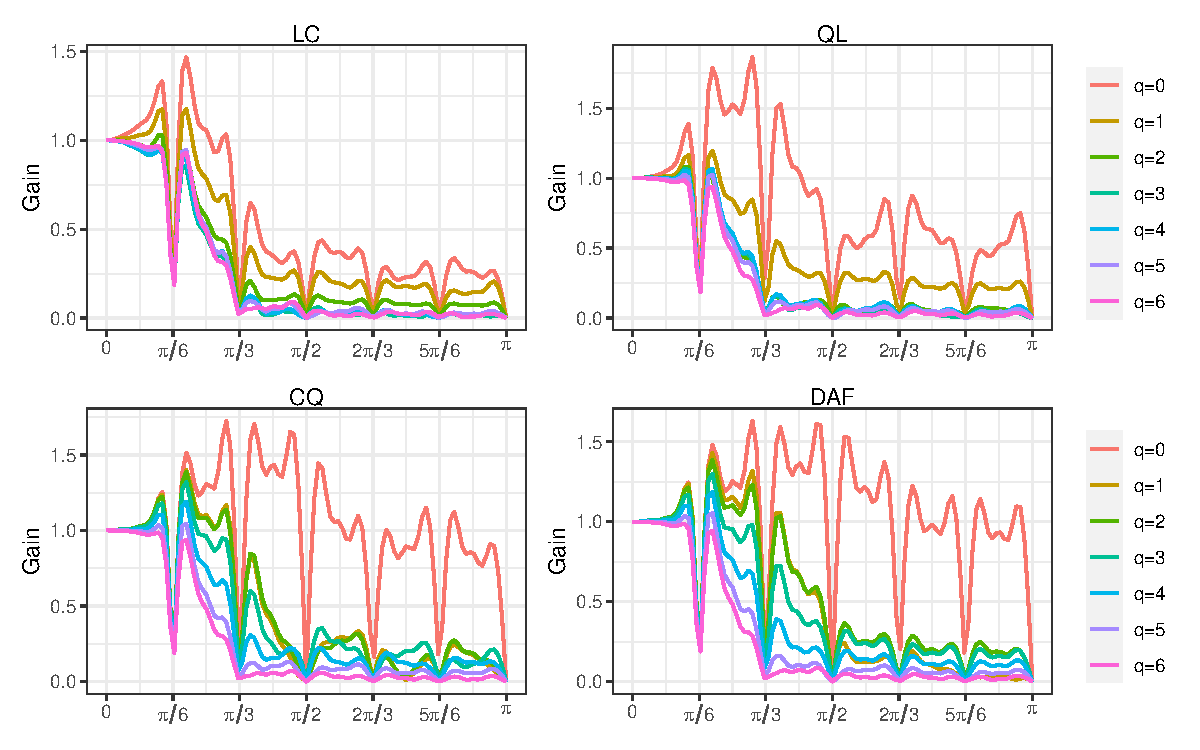
\includegraphics[width=1\linewidth]{img/gain_lp} \end{center}
\end{frame}

\begin{frame}[fragile]{ex \texttt{rjd3filters} : filtres X-11}
\protect\hypertarget{ex-rjd3filters-filtres-x-11-1}{}
\begin{Shaded}
\begin{Highlighting}[]
\NormalTok{knitr}\SpecialCharTok{::}\FunctionTok{include\_graphics}\NormalTok{(}\StringTok{"img/gain\_autres.pdf"}\NormalTok{)}
\end{Highlighting}
\end{Shaded}

\begin{center}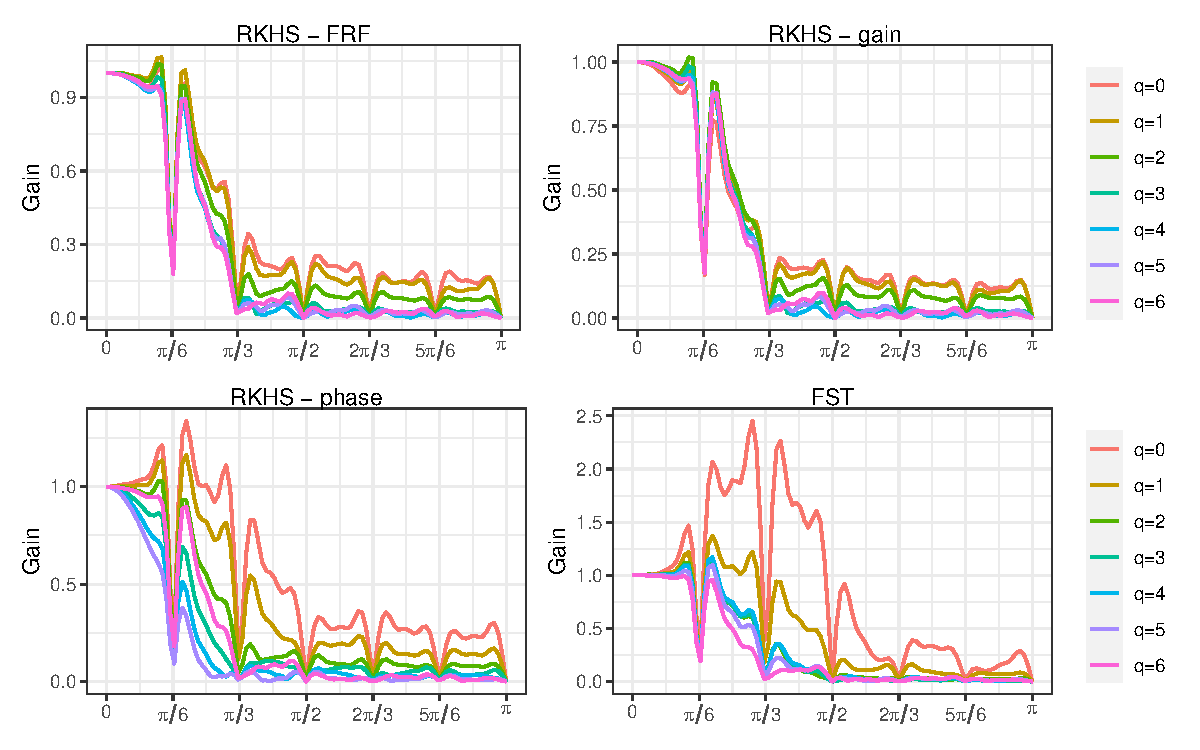
\includegraphics[width=1\linewidth]{img/gain_autres} \end{center}
\end{frame}

\hypertarget{et-maintenant}{%
\section{Et maintenant ?}\label{et-maintenant}}

\begin{frame}{Suite de l'étude actuelle}
\protect\hypertarget{suite-de-luxe9tude-actuelle}{}
Document de travail en cours de finalisation

Soumission au JOS autour de la paramétrisation locale

Objectif d'une soumission d'un article ``informatique'' au Journal of
Statistical Software

\pause

Reste une autre étude. Projet de recherche :

\begin{quote}
Le second objectif de ce projet sera d'étudier l'impact de points
atypiques sur les différentes méthodes d'extraction de cycle et sur la
détection des points de retournement.
\end{quote}

\begin{quote}
Cet objectif d'étude d'impact des points atypiques amènera à également
s'intéresser à l'utilisation de méthodes robustes pour l'estimation de
la tendance-cycle, par exemple par l'utilisation de médianes mobiles
(Tukey, 1971), mais aussi dans les autres étapes de la
désaisonnalisation (pré-ajustement, estimation de la composante
saisonnière, etc.).
\end{quote}
\end{frame}

\begin{frame}[noframenumbering]{Merci pour votre attention}
\protect\hypertarget{merci-pour-votre-attention}{}
\end{frame}

\end{document}
